\documentclass{article}
\usepackage[utf8]{inputenc}
\usepackage{amsmath}
\usepackage{amssymb}
\usepackage{mhchem}
\usepackage{graphicx}
\usepackage{wrapfig}
\usepackage{float}
\usepackage[format=plain, indention=0.5cm, aboveskip=0.1cm, belowskip=0cm]{caption}
\usepackage[paper=a4paper,left=35mm,right=35mm,top=35mm,bottom=35mm]{geometry}
\usepackage[ngerman]{babel}
\usepackage{csvsimple}
\usepackage{array}
\usepackage{booktabs}
\usepackage{siunitx}
\usepackage{physics}
\usepackage{hyperref}
\usepackage[bottom]{footmisc}
\usepackage{textcomp}

\title{\huge T02: Gamma spectroscopy and Compton scattering}
\author{\Large Jonas Colve, Matrikelnr. 377593\\ \Large Anna Stollenwerk, Matrikelnr. 381103 \\Gruppe 43}
\date{10.4.20}

\begin{document}
\renewcommand{\figurename}{Fig.}
\renewcommand{\tablename}{Tab.}

\maketitle
\newpage



\tableofcontents

\newpage

\section{Introduction}
In this experiment different interactions between photons and matter are observed.\\
The photons have an energy $E_\gamma$ between 5keV and 2MeV. For this energy range there mainly happen three different interactions, dependent on the energy $E_\gamma$ the photon possesses.
Furthermore the relative strength of these interactions depends on the binding energy $E_B$ of the electrons in the material which one happens. The interactions are
\begin{enumerate}
    \item $E_\gamma > E_B$ : Photoelectric effect ($\sigma \propto \frac{Z^5}{E^x}$, x = 1 for $E_\gamma \gg m_ec^2$, x = 7/2 for $E_\gamma \ll m_ec^2$)
    \item $E_\gamma \gg E_B$ : Compton scattering ($\sigma \propto Z\cdot f(E_\gamma)$, $f'(x)<0$)
    \item $E_\gamma > 2m_e c^2(1+ \frac{m_e}{M})$: Pair production ($\sigma \propto Z\ln(E_\gamma)$)
\end{enumerate}
The photoelectric effect means that an electron near to the nucleus is kicked out of the atomic shell, with $E_{kin} = E_\gamma - E_B$.
Another electron from a higher energy level within the shell can occupy the empty state left behind by the other electron. This transition emits a new photon.
If only the electron is detected, a peak at the kinetic energy will occur. 
If the electron and the photon are detected, the measured energy will be $E_\gamma$.\\
Compton scattering is an elastic collision between a photon and a quasi-free electron. Both have a continuous energy spectrum with
\begin{equation}
    E_\gamma' = E_\gamma \frac{1}{1+a(1-\cos{\theta})} \mbox{ , } E_e = E_\gamma - E_\gamma' \mbox{ , } a = \frac{E_\gamma}{m_ec^2}
    \label{eq_Compton}
\end{equation}
So the energy depends of the scattering angle. The maximal energy of the electron at $\theta = 180^\circ$ is called Compton energy $E_C$.
So the spectrum as a sharp edge at $E_C$. 
Another edge in the spectrum is at $E_R = E_\gamma'$, which is occasioned by Compton scattering outside the scintillator material.
The differential cross-section of Compton scattering is
\begin{equation}
    \frac{d\sigma}{d\Omega} = \frac{\alpha^2\lambda_e^2}{8\pi^2\rho^2}(\rho+\frac{1}{\rho}-\sin{\theta}^2) \mbox{ , } \rho = \frac{E_\gamma}{E_\gamma'}
    \label{diff_theo}
\end{equation}
with $\lambda_e =$ Compton wavelength and $\alpha =$ fine-structure constant.\\
A photon decaying in an electron and a positron is called pair production. 
If those two get decelerated, they form positronium which decays in two to three photons, depending on their spins.
According to how many of those photons are detected, different energies are measured in the scintillator. 
If all of them are detected, one measures $E_\gamma$, but only $E_{esc}^{(1)} = E_\gamma-m_ec^2$ if one escapes and $E_{esc}^{(2)} = E_\gamma-2m_ec^2$ if both do.
    \footnotetext{Source: \url{https://institut2a.physik.rwth-aachen.de/de/teaching/praktikum/Anleitungen/T02_English.pdf}}
    \begin{figure}[H]
       \centering
        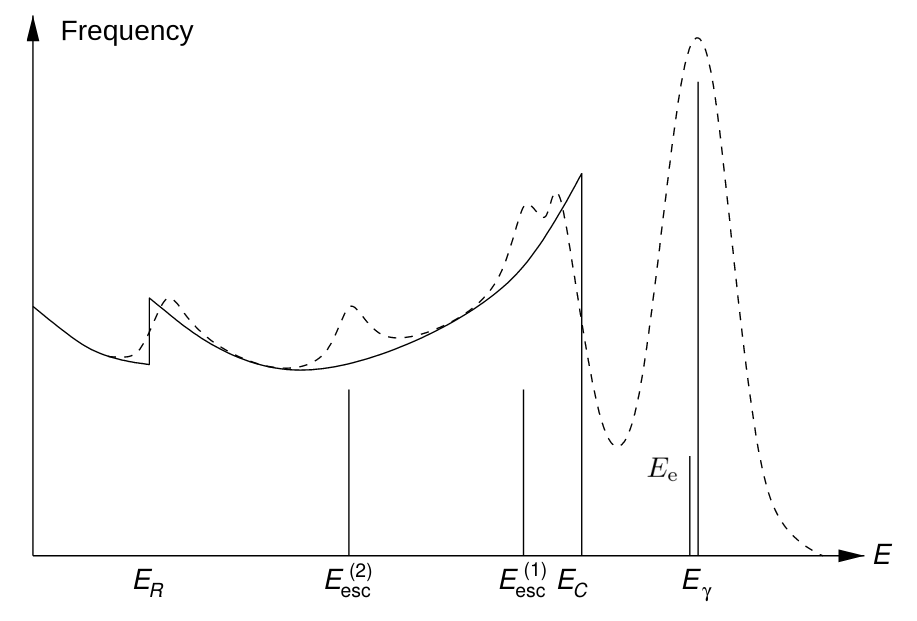
\includegraphics[width=0.6\textwidth]{Bilder/spectrum.png}
        \caption{The energy spectrum including the three main interactions of photons and matter. The theoretical curve is drawn through, the experimental one is shown dashed\footnotemark}
        \label{spec_pic}
    \end{figure}

The resulting spectrum is shown in fig.(\ref{spec_pic}).
The deviation between the theoretical and experimental curve comes from the finite energy resolution of the detector. 
It is given by 
\begin{equation*}
    \frac{\Delta E}{E} = \sqrt{a^2 + \frac{b^2}{E}}
\end{equation*}
where $\frac{b}{\sqrt{E}}$ is the result of the Poisson statistical creation of the scintillator photons. $a$ describes other influences.\\
Another property of the detector is the efficiency $\epsilon = m/m_0$, it can be calculated from the counting rate
\begin{equation}
    m = \underbrace{\frac{A\cdot I_\gamma}{4\pi r^2}}_{\mbox{particle flux}}F_D\cdot\epsilon
    \label{eff}
\end{equation}
with $F_D =$ detection area. $m_0$ is the rate of all incoming particles.\\
The counting rate can also be used to measure the cross section of Compton scattering, using
\begin{equation}
    m = \frac{A\cdot I_\gamma}{4\pi r_0^2}\eta\cdot\epsilon\cdot N_e\frac{d\sigma}{d\Omega}\frac{F_D}{r^2}
    \label{diff_cross}
\end{equation}
, with $\eta$ as the absorption in air and the scattering body, $N_e$ the number of electrons in the scattering body, $r_0$ the distance between the source and the scattering body $r$ the distance between the scattering body and the detector.\\
The detector consists of a scintillating material, a photo-multiplier, some pulse logic and an MCA. 
The emitted photons are converted to an electric signal by the photo-multiplier with is amplified and shaped. Then it is analysed by the multi channel analyser, with sorts the different signals by their pulse height.

\newpage
\section{Energy spectroscopy}
\begin{figure}[H]
       \centering
        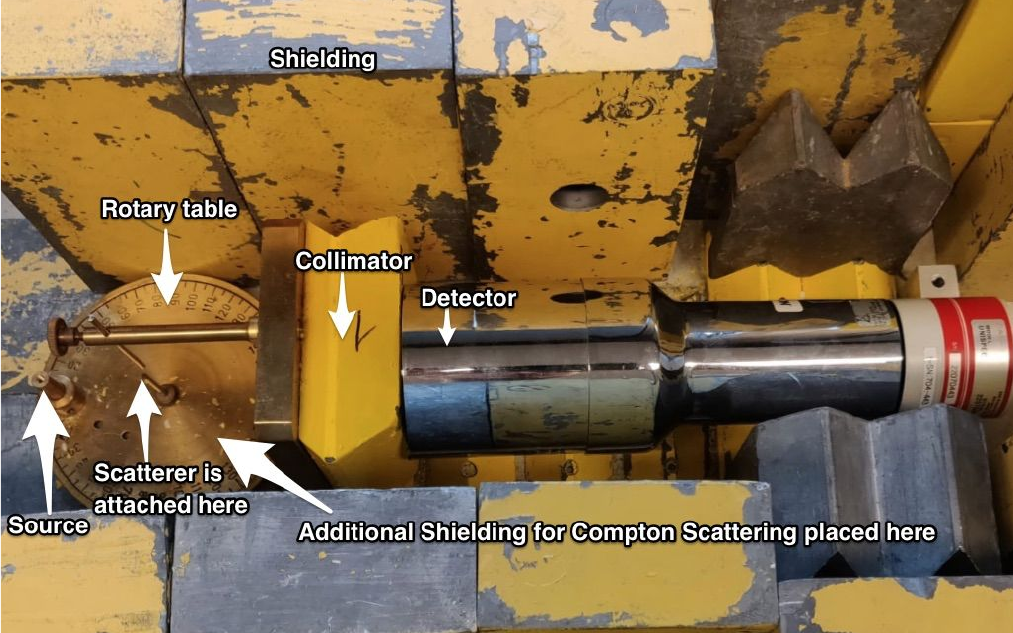
\includegraphics[width=0.7\textwidth]{Bilder/Conventional_Setup.png}
        \caption{Conventional geometry, for the spectroscopy the angle between the source and the detector is 0$^\circ$}
        \label{conventional}
\end{figure}
To measure the energy spectrum, seen in fig.(\ref{spec_pic}), a source is placed in front of the detector. 
The setup can be seen in fig.(\ref{conventional}).
The sides of the detecting scintillator material is shielded by a collimator to minimize the measured ambient radiation. 
Around the whole setup is shielding made of lead to protect the experimenters against the radiation of the source.
The used sources are \ce{^{60}Co}, \ce{^{137}Cs}, \ce{^{152}Eu} and \ce{^{22}Na}. The following histograms show the measured spectra. The noise measurement is already subtracted. The measurement time is 10 minutes.
\begin{figure}[H]
       \centering
        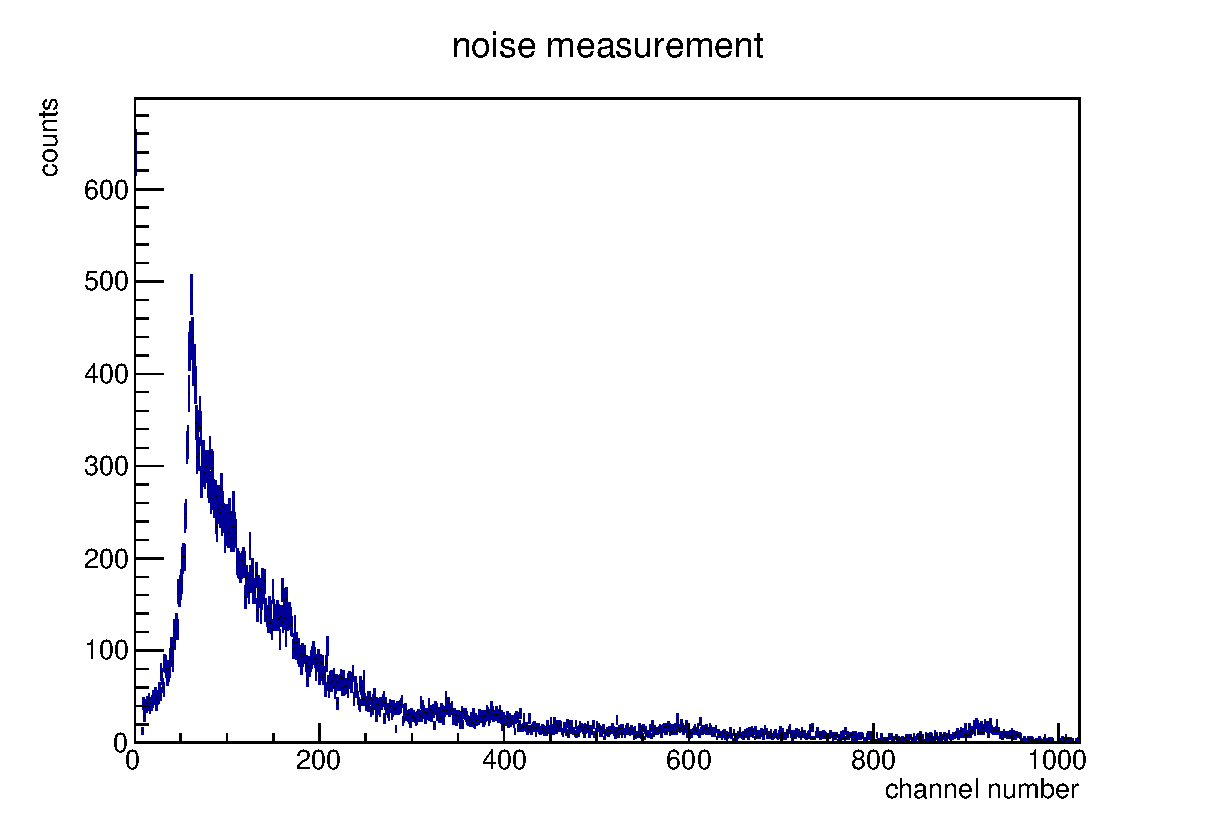
\includegraphics[width=0.85\textwidth]{Graphen/calibrate/uncalib_spectra/noise.eps}
        \caption{Empty measurement of the set up. The spectrum is caused by the continuous and characteristic X-radiation of the lead shielding.}
\end{figure}
\begin{figure}[H]
       \centering
        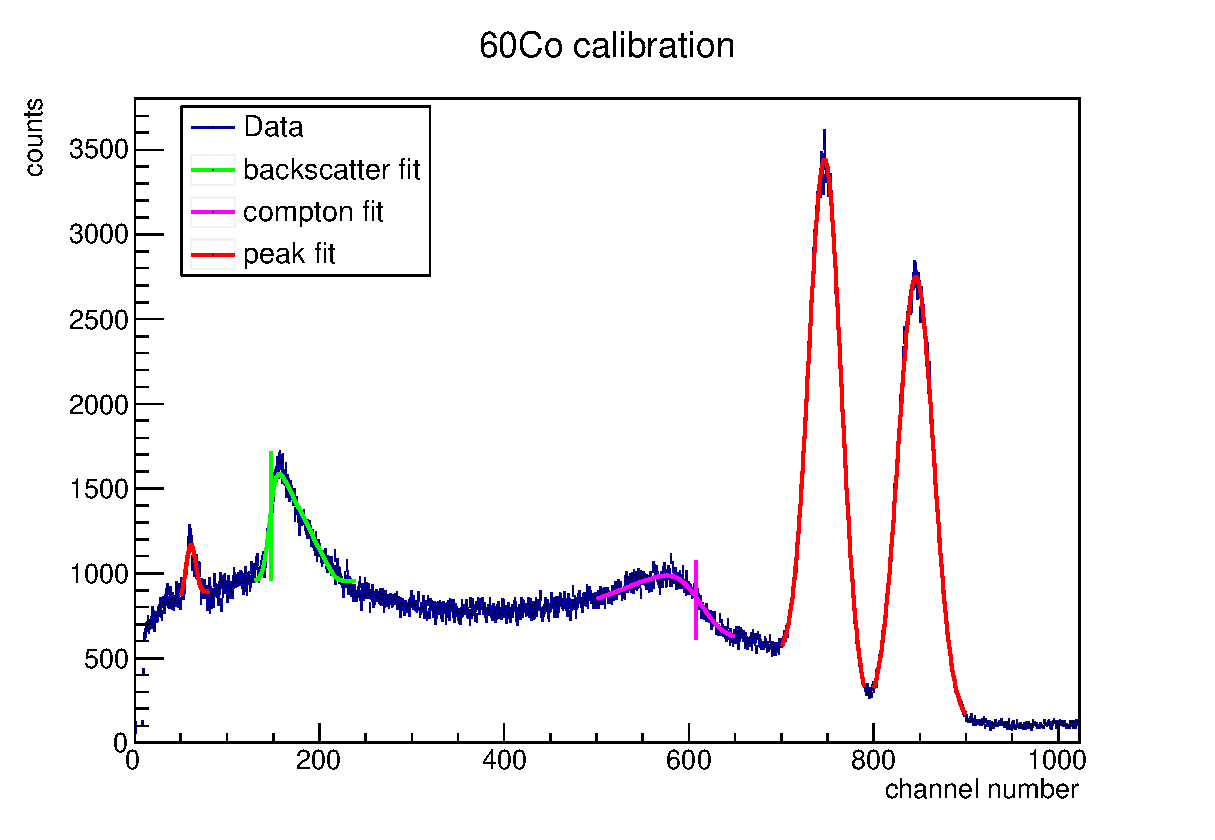
\includegraphics[width=0.85\textwidth]{Graphen/calibrate/uncalib_spectra/60Co.eps}
        \caption{Measurement of \ce{^{60}Co}.The peak on the right arises from the gamma radiation of the B- decay with a half life of 10.467 M and 5.2714 Y.\\ 
        The next peaks occurs from the gamma rays of the B- decay with a half life of 5.2714 Y. The marked Compton edge and back-scatter peak belong to it, because the distance between the photo peak and the Compton edge has the same size as the distance between the back-scatter peak and the y-axis.\\
        The small peak on the left is determined by the additional X-rays of lead, that are coursed by the radiation of the source. Because of that, the peak is not suppressed by subtracting the noise measurement. }
\end{figure}
\begin{figure}[H]
       \centering
        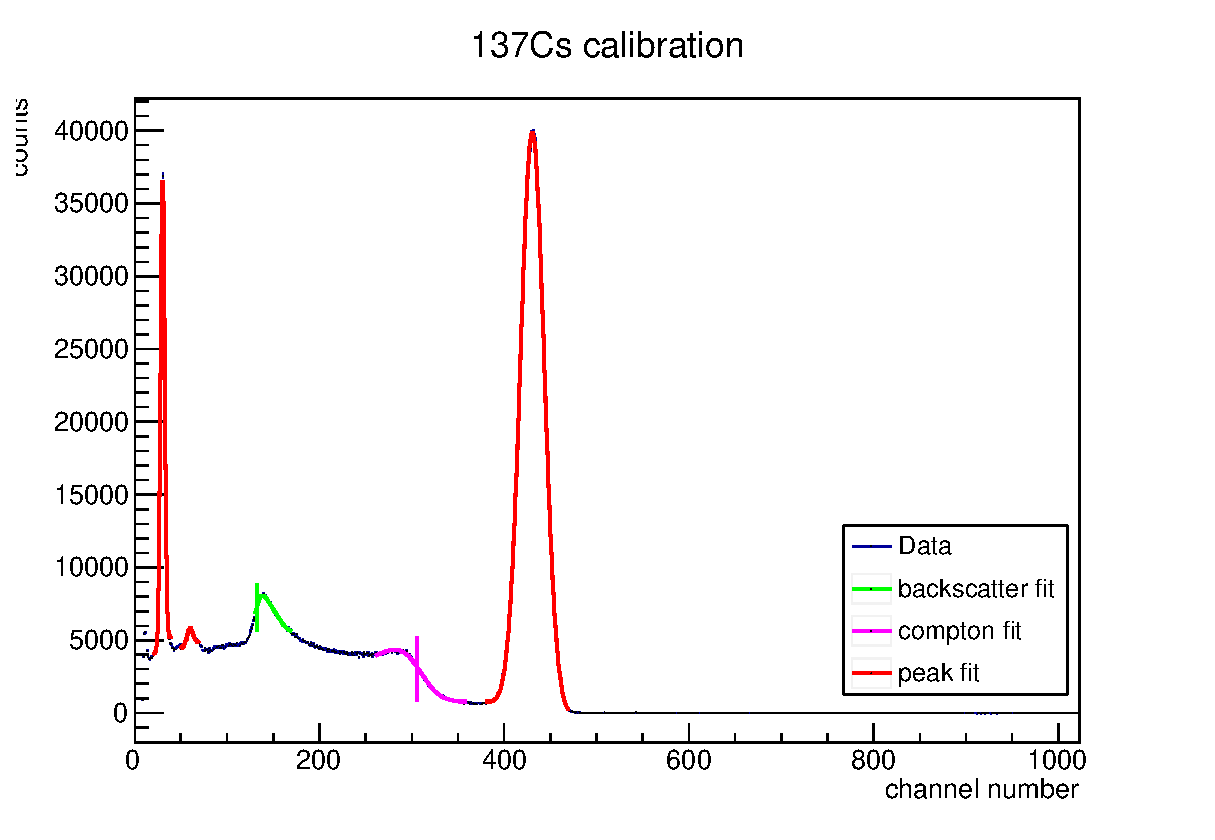
\includegraphics[width=0.85\textwidth]{Graphen/calibrate/uncalib_spectra/137Cs.eps}
        \caption{Measurement of \ce{^{137}Cs}. The peak on the left is caused by the X-rays of \ce{^{137}Ba}, which is the decay product of B- decay of the source.\\
        Next to it is again the X-radiation peak of lead.\\
        The peak on the right is the photo peak, caused by gamma radiation, also emerged by the B- decay. The associated Compton edge and back-scatter peak are also marked. }
\end{figure}
\begin{figure}[H]
       \centering
        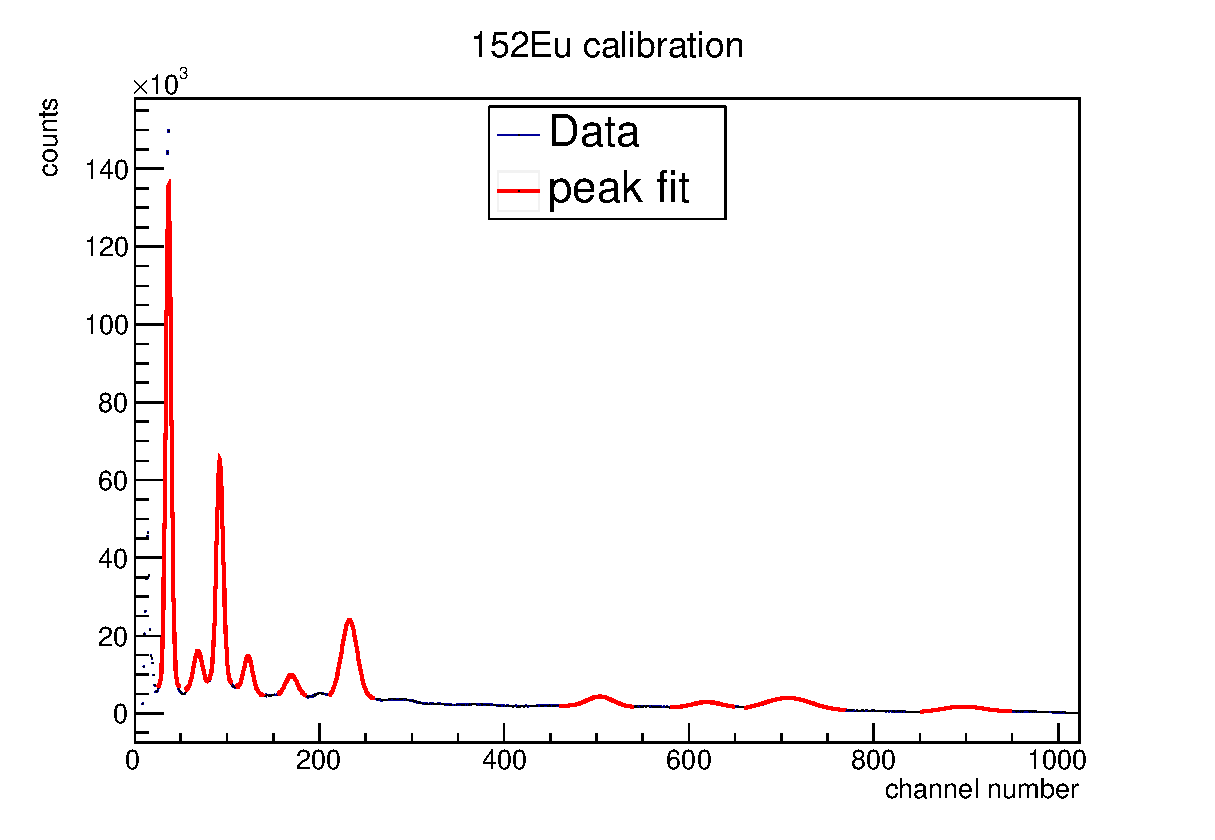
\includegraphics[width=0.85\textwidth]{Graphen/calibrate/uncalib_spectra/152Eu.eps}
        \caption{Measurement of \ce{^{152}Eu}. Because it decays in various ways, there are no Compton edges or back-scatter peaks visible. Due to the fact that the peaks are very close to each other, their corresponding decay is determined after the calibration with the other spectra. This gives from left to }
\end{figure}
\begin{figure}[H]
       \centering
        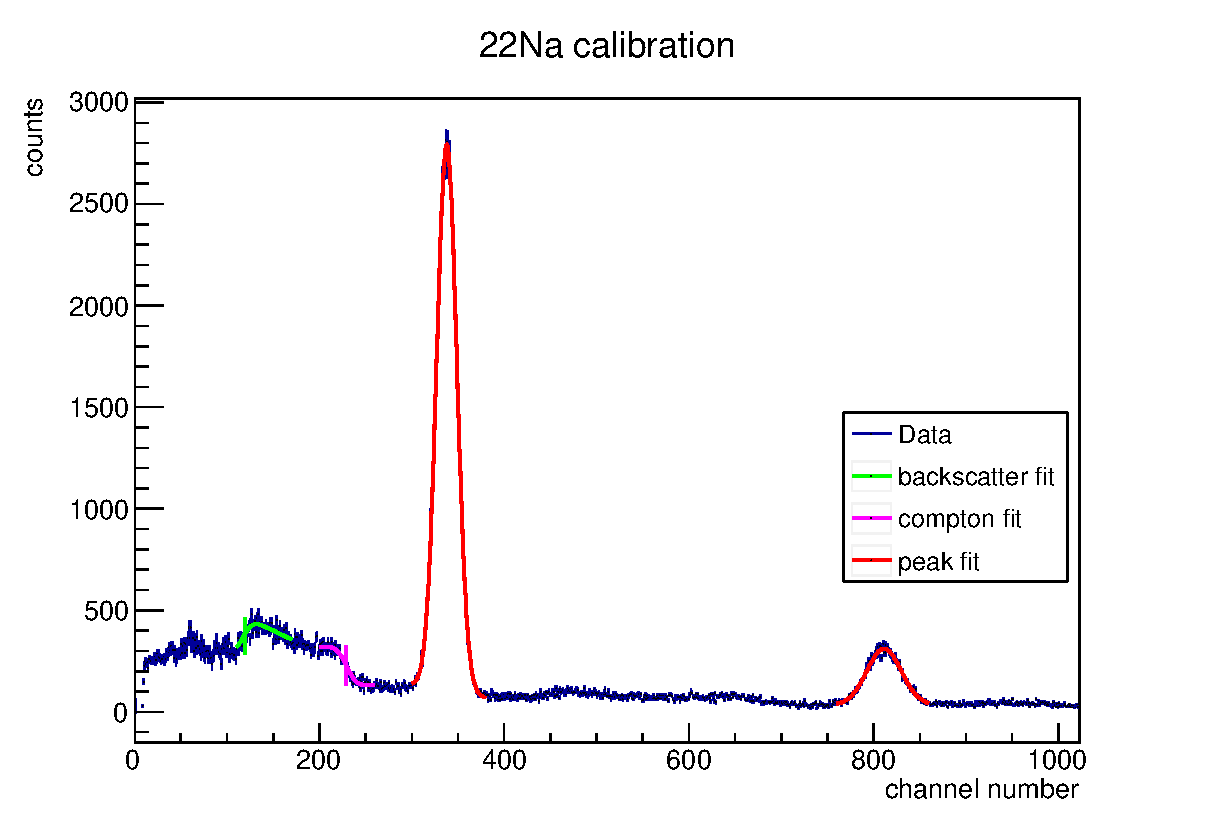
\includegraphics[width=\textwidth]{Graphen/calibrate/uncalib_spectra/22Na.eps}
        \caption{Measurement of \ce{^{22}Na}. The high energetic peak on the right is caused by the gamma radiation of the $\beta+$ decay of this sodium isotope.\\
        The large peak comes from pair production and the emitted positron of the $\beta+$ decay. The Compton edge and back-scatter peak are caused by photons of the same energy.}
\end{figure}

\subsection{Calibration}
To calibrate the MCA, the spectra of known sources are analysed.
The known energies of the photo peaks, Compton edges and back-scatter peaks are plotted against the channel number.
A linear function is fitted to those data points.\\
The positions of the peaks are determined by taking the mean value of the Gaussian distribution fitted to the data segment. To the fitted Gaussian function is also a linear background term added.\\
The positions of the Compton edges are extracted by fitting the convolution of a Gaussian normal distribution and a triangle function\footnotemark against the data. One assumes a constant background.
\footnotetext{See appendix for formula}
For back-scatter peaks this distribution is mirrored around the y-axis.\\
One uses the the position of triangle edge as the Compton or back-scatter edge resp.
Using this Method one can use a linear regression to obtain a first calibration, which then can be used to match the peaks of the \ce{^{152}Eu} spectrum to literature values:
\begin{figure}[H]
    \centering
    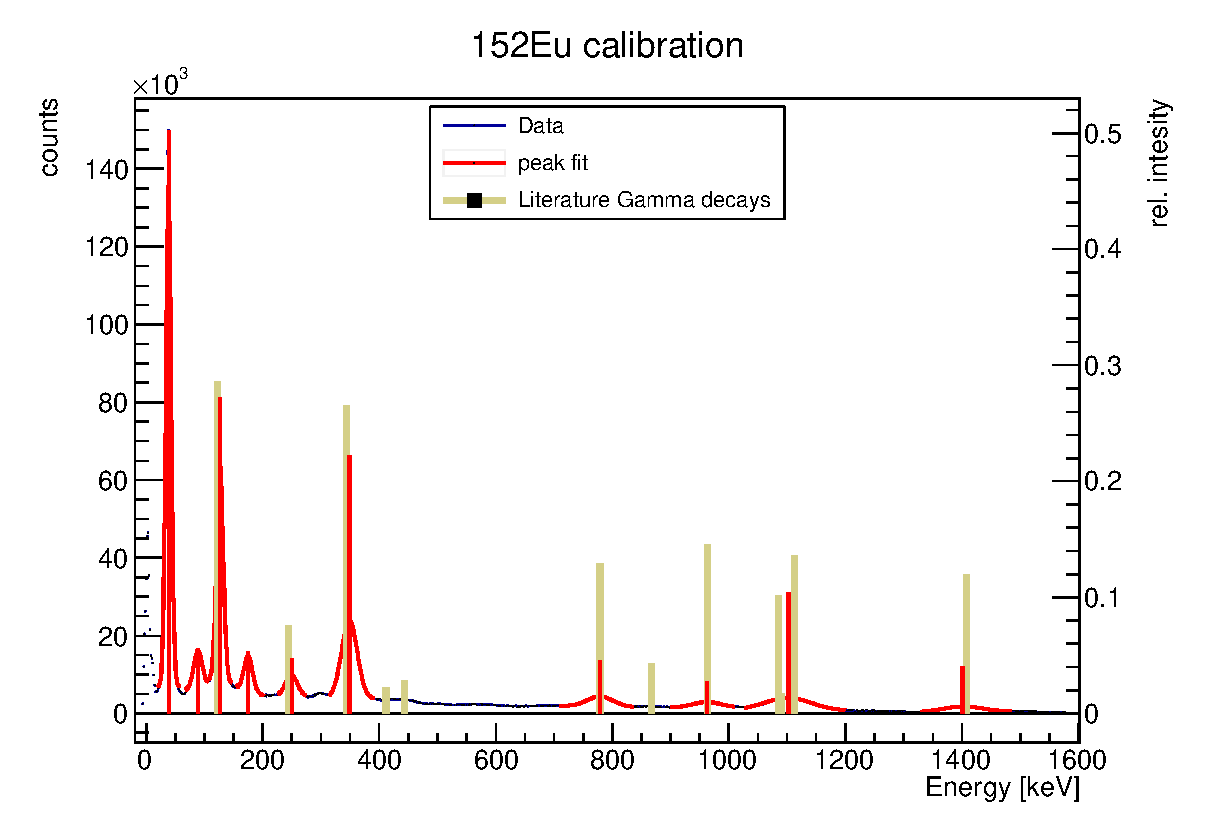
\includegraphics[width=\textwidth]{Graphen/eu/eu.eps}
    \caption{The \ce{^{152}Eu} spectrum, the peak positions and literature energies with relative intensities }
    \label{eu_match}
\end{figure}
The peaks, that can be clearly matched to a literature energy are then added to the calibration. It is apparent that the peak at $E=1102 keV$ contains two different gamma energies, so one assumes $E_{lit}=\frac{E_1+E_2}{2} \pm \frac{|E_1-E_2|}{2}$ for its energy.
The resulting graphs and the linear regression for the final calibration are shown in fig.(\ref{cali})
\begin{figure}[H]
    \centering
    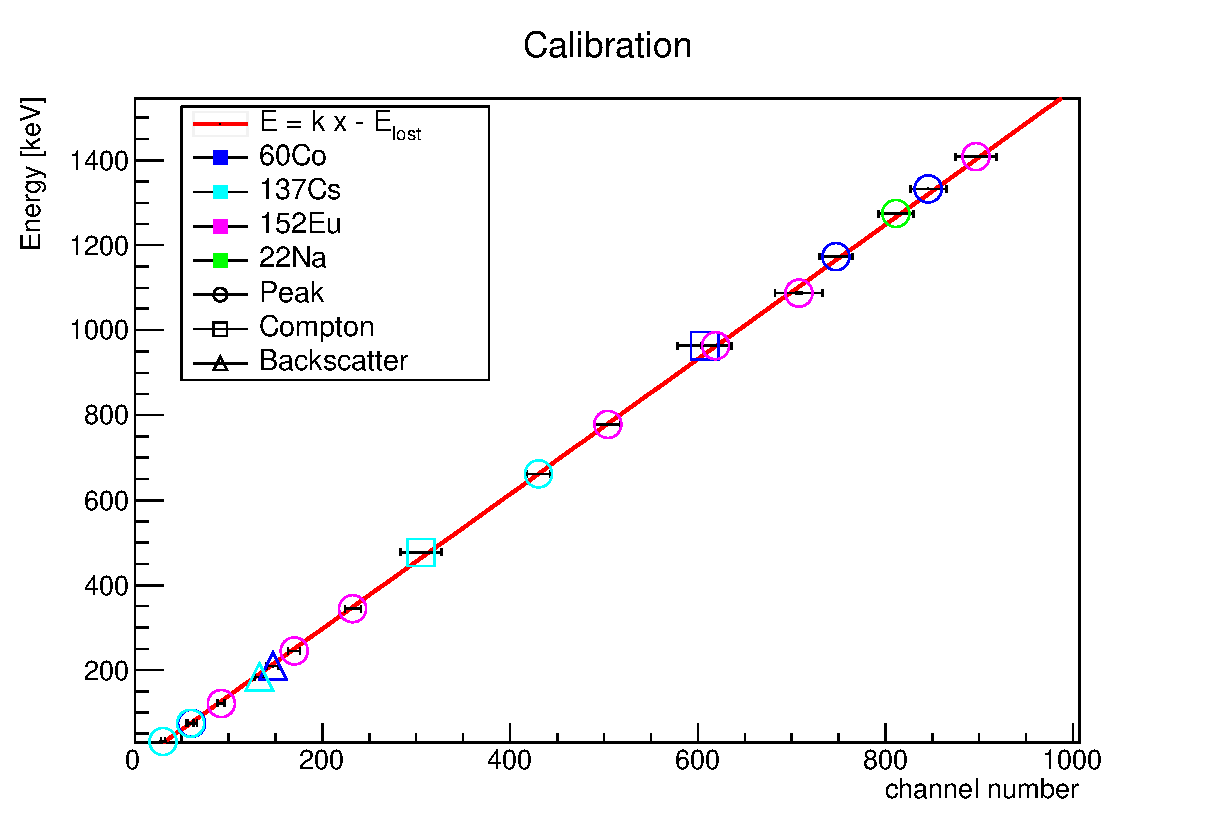
\includegraphics[width=0.8\textwidth]{Graphen/calibrate/calibration_lin_reg.eps}
    \caption{Linear fit to determine the calibration factor and offset}
    \label{cali}
\end{figure}

\begin{table}[H]
    \centering
    \caption{Parameters of the calibration}
    \begin{tabular}{l|l}
    
        $E_{lost}$[keV] & $19.6 \pm 2.6$ \\\hline
        $k$[keV] & $1.59 \pm 0.02$ \\\hline
        $\chi^2/N_{dF}$ & 0.244\\
    
    \end{tabular}
\end{table}
Now with this function, the energy of the following measurements can be calculated. The error of the calibration is taken as systematic error in further calculations. 

\subsection{Energy resolution}
To measure the energy resolution of the detector for different energies the width of the photo peaks is determined.
For this one uses the standard deviation given by Gauss fits similar to the ones used for the calibration.
The peak of \ce{^{152}Eu} containing two different decays must be excluded, since its width is increased above the uncertainty caused by the detector.

\begin{figure}[H]
    \centering
    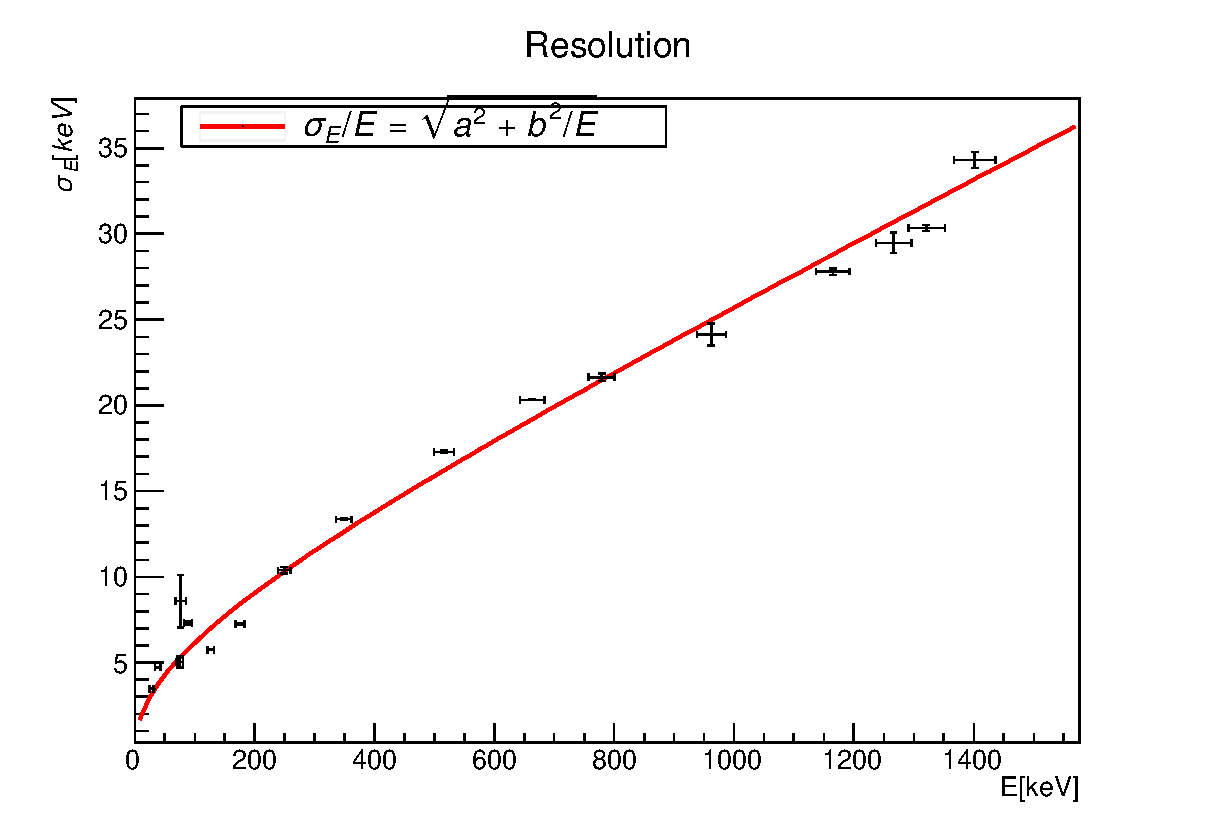
\includegraphics[width=\textwidth]{Graphen/resolution/resolution.eps}
    \caption{Plot of standard deviation against energy and fit of the form $\Delta E = E\qty(a \bigoplus \frac{b}{\sqrt{E}} )$}
    \label{res}
\end{figure}
\begin{table}[H]
    \centering
    \caption{Results for the energy resolution}
    \begin{tabular}{l|l}
        $a$ & $(17.7 \pm 0.5)\cdot10^-3$ \\\hline
        $b$ & $(590.0 \pm 9.6)\cdot10^-3\sqrt{keV}$ \\\hline
        $\chi^2/N_{dF}$ & 11.5\\
    \end{tabular}
\end{table}
One can see from the graph, the resolution matches the theoretical shape quite well, although the $\frac{\chi^2}{N_{dF}}$ indicates an underestimation of the errors by the peak fits.
All in all the resolution is in the per mile to percent range.
Notable is also, that one can estimate the energy of the scintillator photons through the Poisson error $b$ via:
\begin{align*}
    \frac{\sigma_N}{N} &= \frac{1}{\sqrt{N}} = \frac{b}{\sqrt{E}}\\
    \frac{E}{N} = b^2 = (348.1 \pm 11.3)eV
\end{align*}
This energy is however to large for scintilator photons, which are usually in around the energies of visible light.
This leads to the hypothesis, that some secondary effect is also affecting the resolution in a poisson statistical way.

\subsection{Efficiency of the detector}

The set up is the same as for calibration and the measurement time is also five minutes.
For any geometrical values, the last known digit is taken as error, because the measurement was not performed by the experimenters.
The source is placed in a distance of $r=(17 \pm 1)$ cm in front of the detector.
The exposed detection area is $F_D = (4.91 \pm 0.1)$ cm$^2$.\\
To calculate the efficiency $\epsilon$ of the detector by using eq.(\ref{eff}), the activity of the used source, \ce{^{137}Cs}(OI-797), has to be determined.
In 1.10.2008 it was $A_0 = 24.8$ MBq.\\
The half life is $T_{1/2}=30.04 \pm 0.03$Y. So the current activity is 
\begin{equation*}
    A = A_0\cdot e^{-\frac{\ln{(2)}t}{T_{1/2}}} = (18.586 \pm 0.005)\mbox{MBq}
\end{equation*}
with $t=12.5$Y.\\
The photon yield is $I_\gamma = 0.946 \cdot  0.851 = 0.805$, because \ce{^{137}Cs} decays to 94.4\% to \ce{^{137}Ba^*} which emits a photon with $E_\gamma = (661.657 \pm 0.003)$keV to 85.1\% ,when it populates the ground state.\\
The counting rate $m$ is measured by fitting a Gaussian function with linear background to the appropriate photo peak and integrating the Gaussian function with the calculated parameters. With this method, the background is ignored and the blurring of the peak is taken in to account. The result has to be divided by the measurement time to get the rate. The calculated parameters for the Gaussian distribution are
\begin{enumerate}
    \item[~]amplitude: $A_G = 98390.5643 \pm 72.4652$
    \item[~]mean value: $\mu = 660.0099 \pm 0.01366$ keV
    \item[~]standard deviation: $\sigma = 20.0913 \pm 0.0125$ keV
\end{enumerate}
The integration of the Gaussian function gives
\begin{equation*}
    m = \frac{A_G\cdot\sigma\sqrt{2\pi}}{T} 
\end{equation*}
Using those values and Gaussian error propagation, the result for the counting rate is
\begin{equation*}
    m = (8258.4780 \pm  7.9745)/\mbox{s}
\end{equation*}
with $T = 600$ s. So the efficiency is
\begin{equation*}
    \epsilon = \frac{4\pi r^2 m}{A\cdot I_\gamma F_D} = 0.4107  \pm  0.02557
\end{equation*}
This value is realistic for the used scintillator, so the detector is sensitive enough to measure rates with it.

\subsection{Electron mass}
\begin{figure}[H]
    \centering
    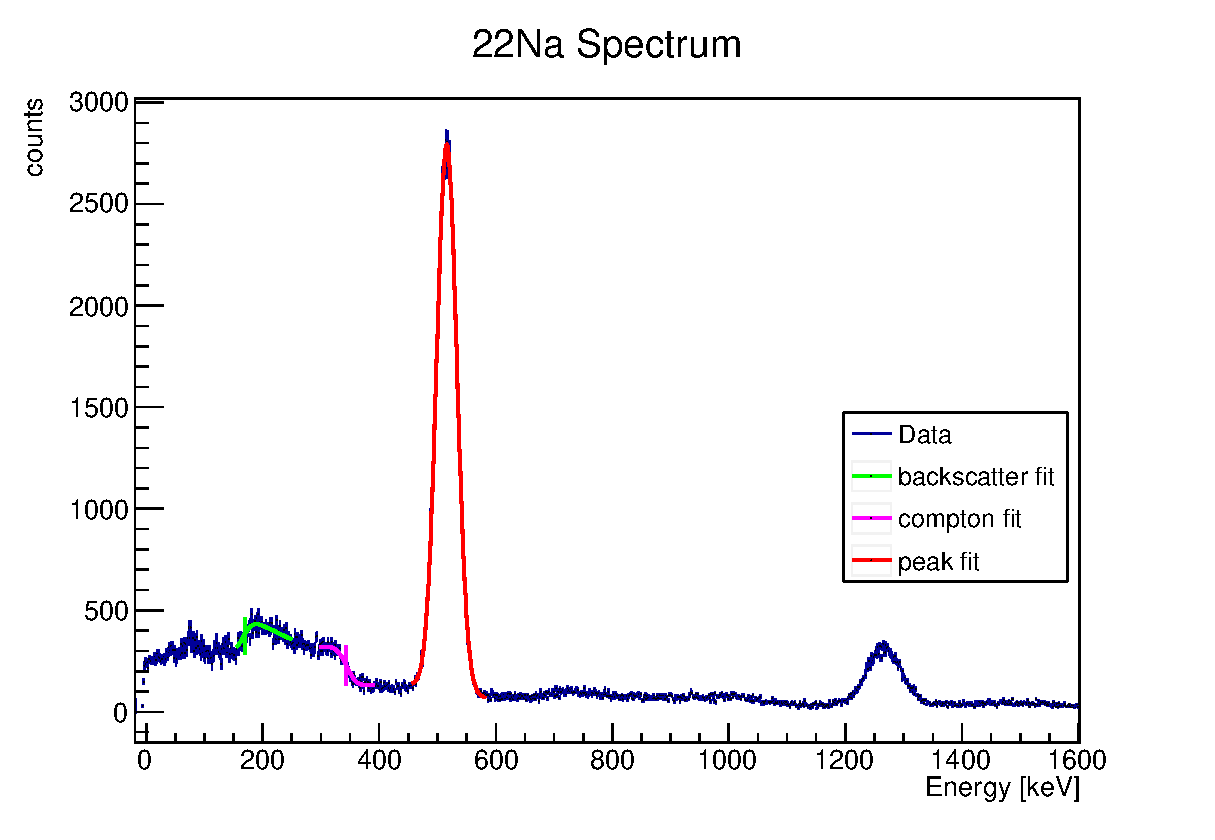
\includegraphics[width=\textwidth]{Graphen/e_mass/e_mass_imp.eps}
    \caption{Fit to the peak and the edges to calculate the electron mass}
    \label{e_mass}
\end{figure}
To calculate the mass of the electron, \ce{^{22}Na} is used. It has a photo peak at this energy, so the position of it will be determined. The peak results from pair production, because sodium emits photons with an energy of about 1274.53 keV, which are energetic enough to produce an electron and positron.
In addition the $\beta+$ decay itself emits a positron which can be detected.\\
Also the Compton edge and back-scatter peak can be used to calculate the electron mass, because
\begin{equation*}
    m_e = 2E_\gamma (\frac{E_\gamma}{E_C}-1) \mbox{ and } m_e = 2E_\gamma\cdot (\frac{E_\gamma}{E_\gamma-E_R}-1)
\end{equation*}
The results are
\begin{table}[H]
    \centering
    \begin{tabular}{l|l|l|l}
         & position [keV] & $\chi^2/N_{dF}$ & $m_e$ [keV] \\\hline
        peak & $515.94 \pm 17.29$ & 1.53 & $515.94 \pm 17.29$ \\\hline
        Compton edge & $342.95 \pm 653.33$ & 1.13 & $520.50\pm 2958.01$\\\hline
        back-scatter peak &  $169.01 \pm 95.98$ & 1.17 & $502.67 \pm 424.63$
    \end{tabular}
\end{table}
One can see that the errors of the Compton energy and back-scatter energy are quite big, because the position is difficult to calculate, even if the fit went well. The weighted average of this values is
\begin{equation*}
    m_e = (515.92 \pm 17.28)\mbox{keV}
\end{equation*}
which is compatible with the expected value of 511.9985\footnotemark keV. 
\footnotetext{\url{https://en.wikipedia.org/wiki/Electron}}

\section{Compton scattering}
In this section, the effects of Compton scattering should be analysed. To measure the radiation at different angles, two different setups are used. The used source is \ce{^{137}Cs} (OI797) \\
The one with conventional geometry is shown in fig.(\ref{conventional}). The scattering angle is changed by putting different lead wedges (50$^\circ$,65$^\circ$,80$^\circ$,95$^\circ$,105$^\circ$ and 135$^\circ$) on the rotary table, so that it blocks radiation with a different scattering angle. The scattering body has a cylindrical shape and is made of aluminium or steel.\\
The geometry of this setup is:
\begin{enumerate}
    \item detection area: $F_D = (4.91 \pm 0.1)$ cm$^2$
    \item distance between source and scattering body: $r_0 = (5\pm 1)$ cm
    \item distance between scattering body and detector: $r = (12 \pm 1)$cm
    \item scattering body diameter: $d = (1.2 \pm 0.1)$cm
    \item scattering body height: $h = (2.1 \pm 0.1)$cm
\end{enumerate}
Again the last known digit is taken as error. A noise measurement is taken for every wedge, because the noise changes if the shielding is modified.
\begin{figure}[H]
    \centering
    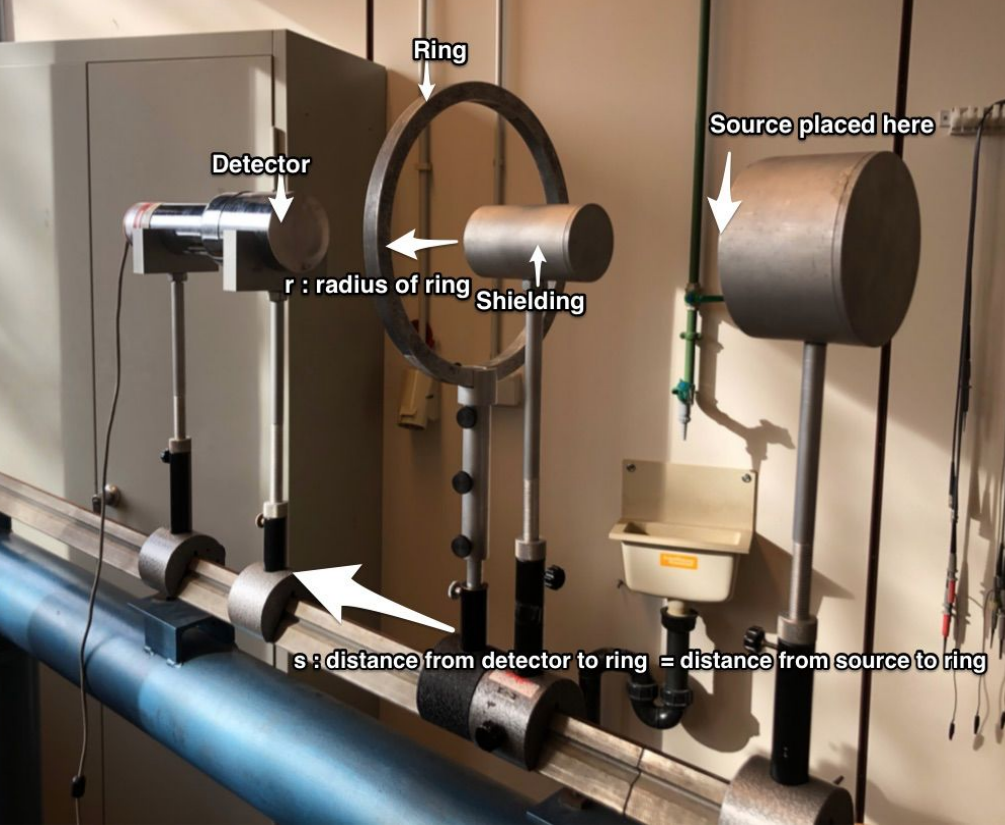
\includegraphics[width=0.6\textwidth]{Bilder/Ring_Setup.png}
    \caption{Ring geometry for measurements of small scattering angles}
    \label{ring}
\end{figure}
The other setup is called ring geometry and is shown in fig.(\ref{ring}). The angle is changed by varying the radius of the ring, that is used as the scattering body. It is made of aluminium. The lead shielding in the middle of the ring blocks the primary radiation. The detection area is $F_D = 51.3 \pm 0.1$cm$^2$.  The scattering angles $\theta$, the distance between source and ring $s$ and the ring radii are
\begin{table}[H]
    \centering
    \begin{tabular}{l|l|l}
        r [cm] & s [cm] & $\theta$  \\\hline
        $11.6 \pm 0.1$ & $25 \pm 1$ & $49.78^\circ \pm 0.85^\circ$ \\\hline
        $8.2 \pm 0.1$ & $25 \pm 1$ & $36.32^\circ\pm 0.63^\circ $ \\\hline
        $6.65 \pm 0.05$ & $25 \pm 1$ & $29.79^\circ\pm 0.51^\circ $ \\\hline
        $11.6 \pm 0.1$ & $70 \pm 1$ &  $ 18.81^\circ\pm 0.33^\circ$  \\\hline
        $6.65 \pm 0.05$ & $70 \pm 1$ & $ 10.85^\circ \pm 0.19^\circ$
    \end{tabular}
\end{table}
the angle is calculated with
\begin{equation*}
    \theta = 2\arctan(\frac{r}{s})
\end{equation*}
The thickness of the ring is ($1.5\pm 0.1)$cm.\\
A noise measurement for $s = (25\pm 1)$cm and $s = (70\pm 1)$cm  is performed, to subtract it from the data with the scattering body.\\
The measured spectra, with and without the noise subtracted, and the fit to the scattered photo peak is shown in the following figures for $\theta = 50^\circ$.
\begin{figure}[H]
    \centering
    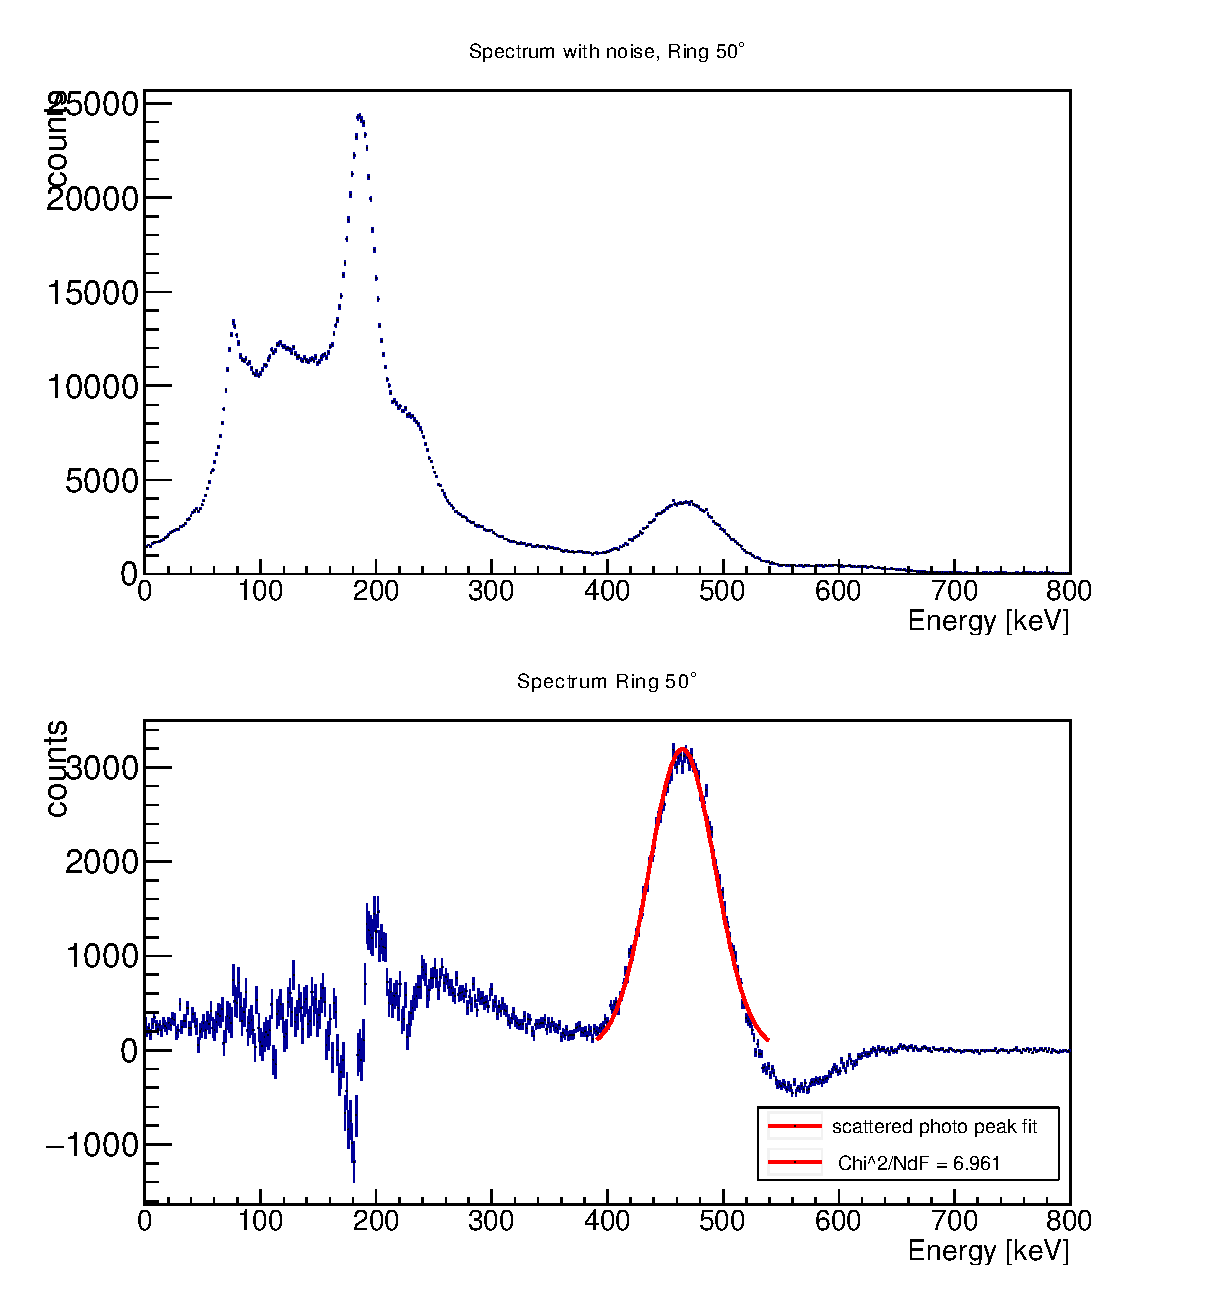
\includegraphics[width=0.9\textwidth]{Graphen/compton_spektren/50grad.eps}
    \caption{Spectrum of the ring geometry. In the upper histogram one can see all detected events.
    In the lower one the noise measurement is subtracted, to make the scattered photon peak visible, to which a Gaussian distribution is fitted. In the ring setup a lot of background radiation is measured, since the shielding is in direct line with the source and the detector. So the bremsstrahlung and the K$_alpha$ line of lead are visible in the upper histogram.}
\end{figure}
\begin{figure}[H]
    \centering
    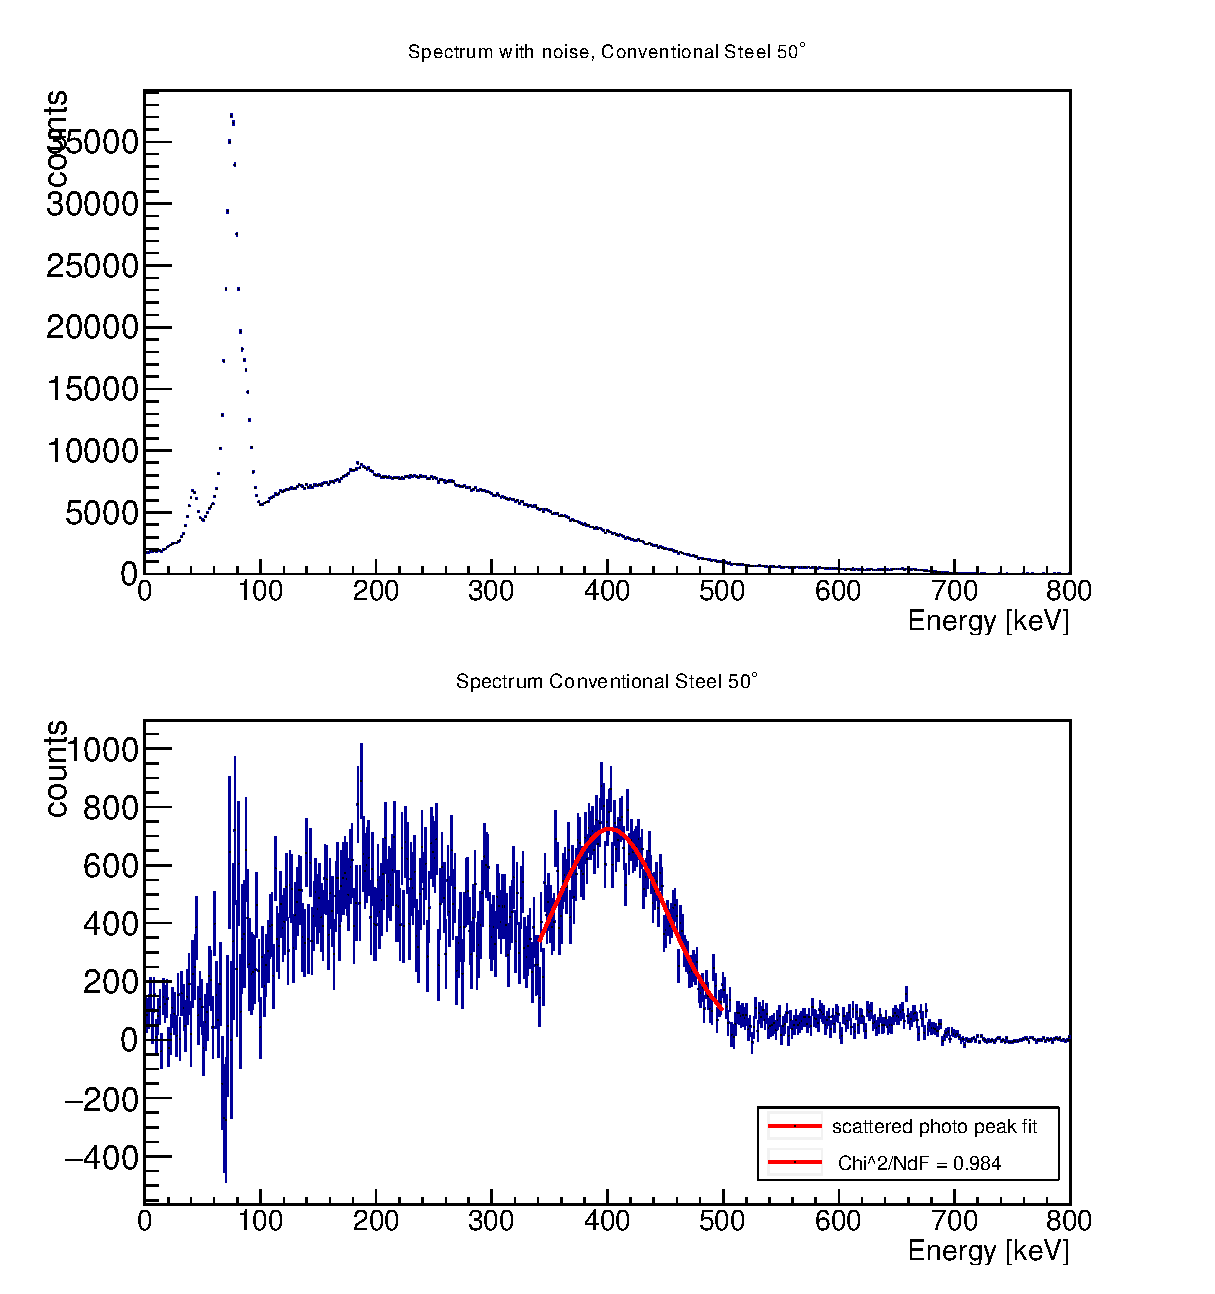
\includegraphics[width=0.9\textwidth]{Graphen/compton_spektren/50Stahl.eps}
    \caption{Spectrum of the conventional geometry with a steel cylinder as scattering body. In the upper histogram one can see a big peak at about 70 keV, which is again caused by the K$_\alpha$ line of lead and also the bremsstrahlung. In the lower one, the $E'_\gamma$ peak is again visible, but it is more difficult to see compared to the ring geometry. For larger angles it is even worse.}
\end{figure}
\begin{figure}[H]
    \centering
    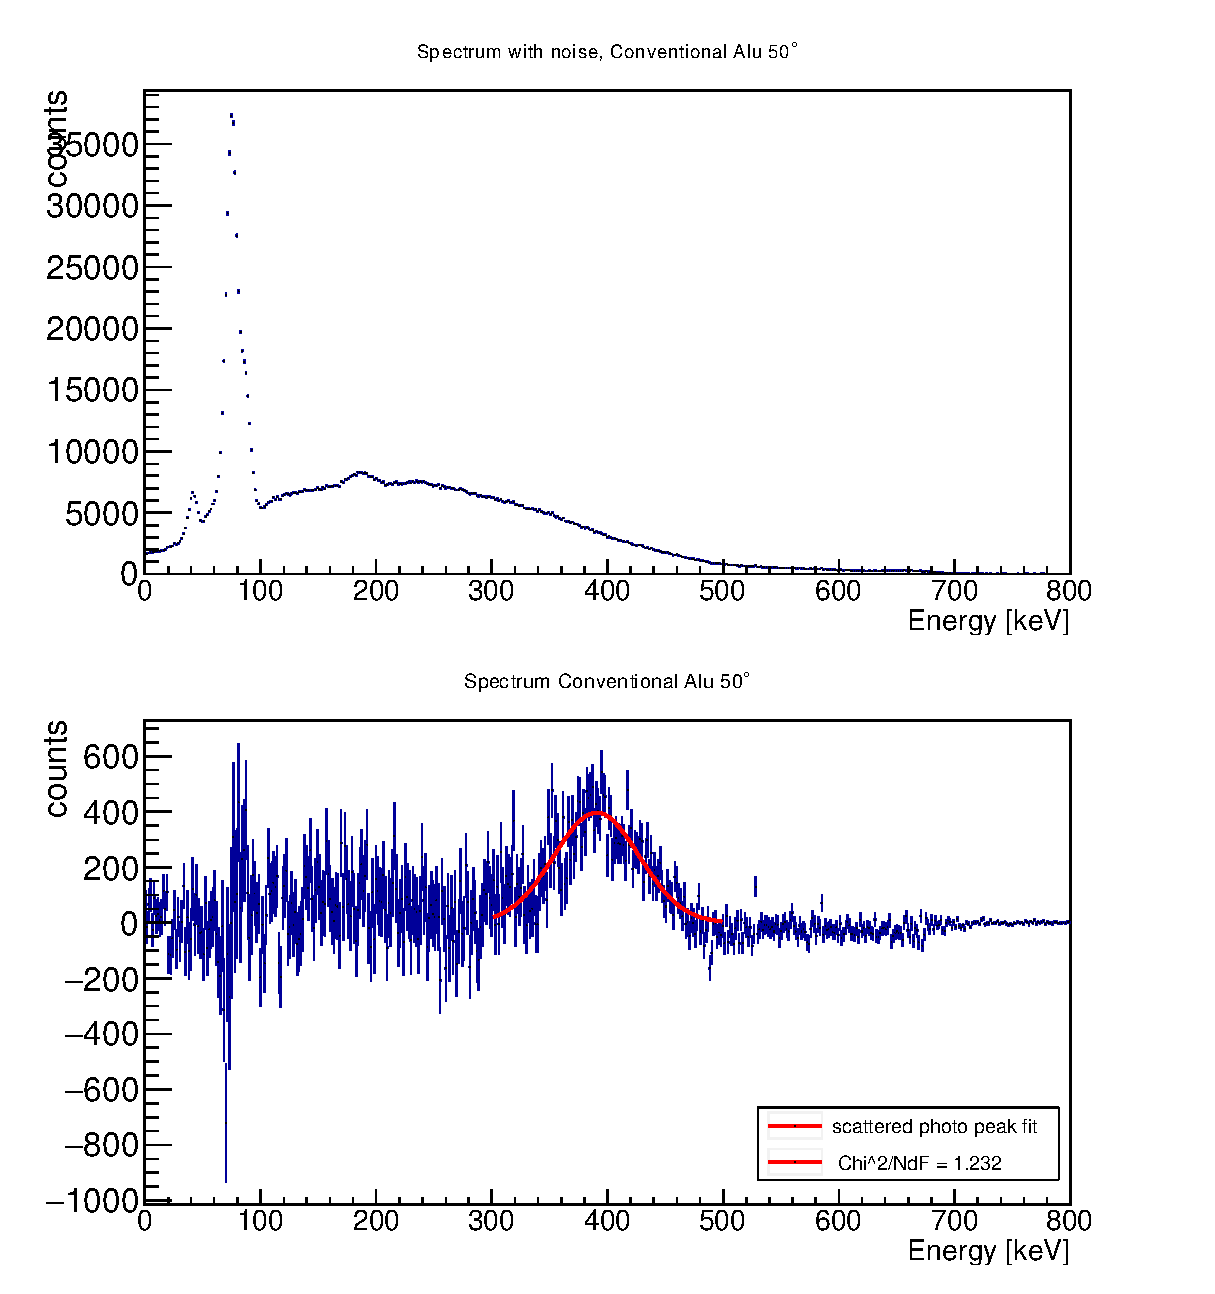
\includegraphics[width=0.9\textwidth]{Graphen/compton_spektren/50Alu.eps}
    \caption{Spectrum of the conventional geometry with a aluminium cylinder as scattering body. Again the K$_\alpha$ line and bremsstrahlung of lead is visible. Here the sought peak is even harder to see compared to the setup with the steel cylinder. }
\end{figure}
The spectra for other angles are visible in the appendix. If the different setups are compared, one can see that the wanted scattered photo peak is way more sharpener in the ring geometry.
It has a better angle resolution, because the background energy is not in the area of the searched peak, like in the spectra of the conventional geometry.
Also the initial radiation is better shielded, so one can even see the wanted peak in the spectrum before deducting the noise.
Unfortunately, the ring geometry can not be used for measuring large angles.

\subsection{Energy of the Compton scattered photon}
\begin{figure}[H]
    \centering
    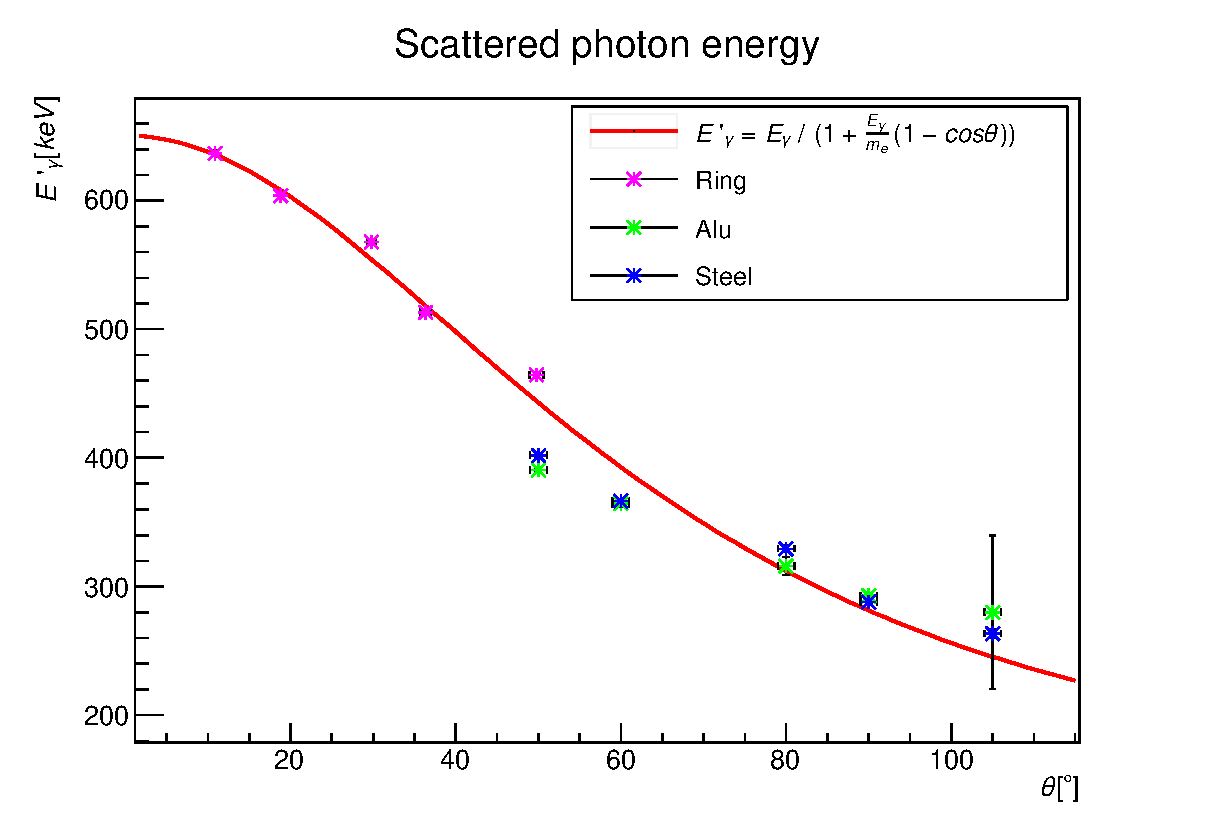
\includegraphics[width=0.9\textwidth]{Graphen/compton_spektren/compton.eps}
    \caption{The fitted parameters of the shown function are $E\gamma$ and $m_e$}
    \label{figure_compton}
\end{figure}
To examine eq.(\ref{eq_Compton}), the energies of the scattered photo peaks are determined by fitting a Gaussian function and taking the mean value. Those values are plotted over the angle.
The results are shown in fig.(\ref{figure_compton}). $E_\gamma$ and $m_e$ are the parameters of the fit. The results are:
\begin{align*}
    & E_\gamma = (654.74 \pm 1.59)\mbox{ keV}\\
    & m_e = (498.40 \pm 6.52)\mbox{ keV}\\
    & \frac{\chi^2}{N_{dF}} = 10.90
\end{align*}
The $\chi^2/N_{dF}$ of the fit is likely to high, because the peaks are hard to find in the conventional setup.
The expected values are $E_{\gamma, theo} = (661.657 \pm 0.003)$ keV and $m_{e, theo} = 510.99895 $ keV. The determined energy is not necessarily compatible, because the error is to small. Nevertheless it is in the right magnitude and quite near to the expectation. The calculated electron mass has a difference of 2$\sigma$, so it is compatible to the theoretical value.\\
So it is likely that the peak energies are determined quite successfully, because the fitted function has parameters quite near to the expected ones.

\subsection{Differential scattering cross-section}
To determine the differential scattering cross-section for different angles eq.(\ref{diff_cross}) is used. To calculate it, a few constants need to be calculated.\\
The activity $A$, photon yield $I_\gamma$ are the same like in the efficiency measurement section. The efficiency $\epsilon$ is the one that is calculated in this section.
Those constants are the same for both setups, because they use the same source and the same detector.\\
The exposed detection areas and the distances between source and detector are different, as mentioned in the setup description.\\
To calculate the counting rate at the scattered photo peak, again the fitted Gaussian function is integrated and divided by the measuring time.\\
The absorption $\eta$ is determined by 
\begin{equation*}
    \eta = e^{-\sum_{material} \mu_{material}(E_{photon})\cdot x_{material}}
\end{equation*}
where $\mu_{material}$ is the attenuation coefficient and $x_{material}$ is the distance traveled in the respective material.
The values of $\mu$ are extracted from the source mentioned in the appendix and linear extrapolated between two values at a time.\\
The amount of electrons in the scattering body is calculated by
\begin{equation*}
    N_e = \frac{V\rho Z}{m_{atom}}
\end{equation*}
where $V$ is the volume of the scattering body, which is calculated with the geometrical data mentioned in the description of the setup.
$\rho$ is the density of the material of the scattering body, $Z$ is the atomic number and $m_{atom}$ the atomic mass.
\begin{figure}[H]
    \centering
    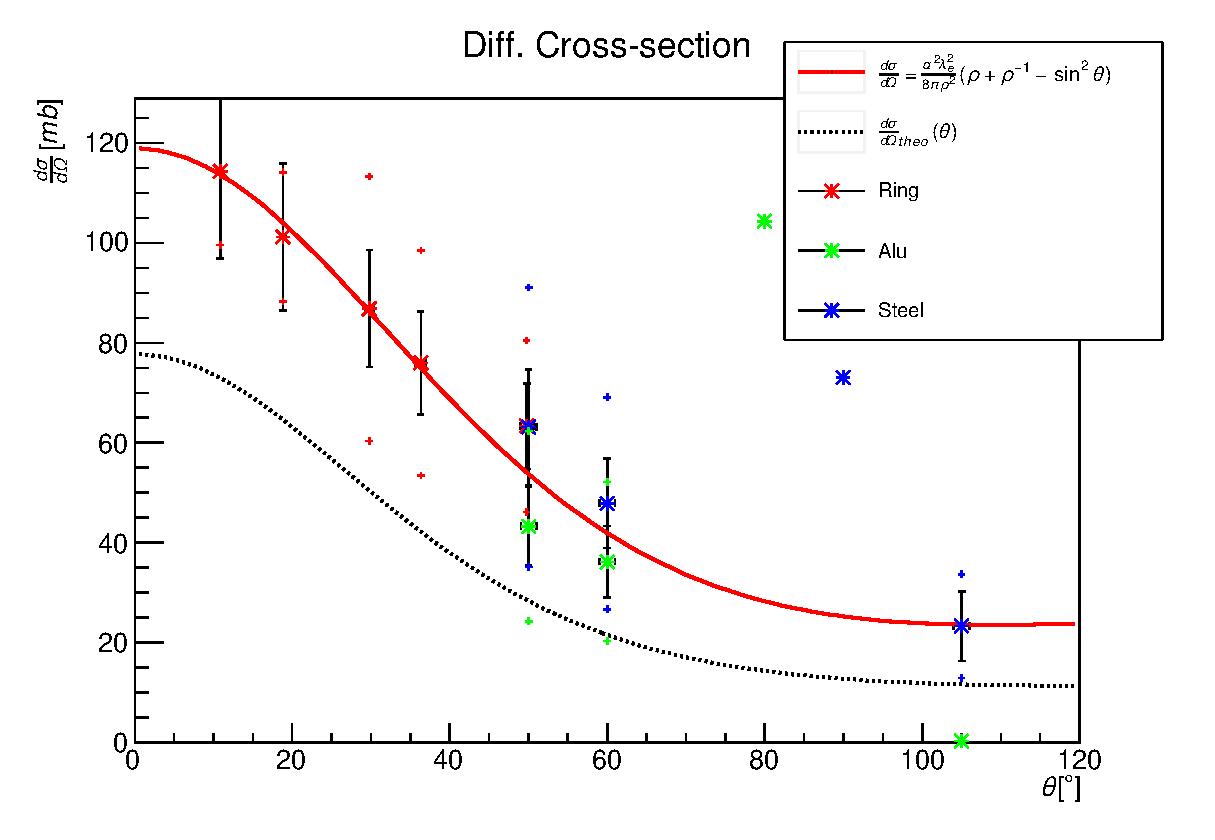
\includegraphics[width=0.9\textwidth]{Graphen/cross-section/diff_cross_Ring_Alu_Steel_.eps}
    \caption{Red: function with fitted amplitude $A = \frac{\alpha^2\lambda^2_e}{8\pi}$ and $ a = E_\gamma / m_e$, black: theoretical values for the amplitude and $a$. The dots above and underneath the normal error bars represent the systematical error.}
    \label{diff_cross_all}
\end{figure}
The result for all determined peaks is shown in fig.(\ref{diff_cross_all}).
The calculated data points are compared to the theoretical curve, given by eq.(\ref{diff_theo}).
For a more detailed analysis, the factor $A$ and $a = E_\gamma / m_e$ where regarded as fit parameters, to compare their differences of the literature values.
The measurements at $80^\circ$ and $90^\circ$ are excluded from this fit, since they deviate extremely from the rest of the data. The most likely cause for this can be seen in \ref{80_alu}, where the peak almost completely disappears in the noise, increasing the standard deviation and therefore the counting rate massively.
Also the $105^\circ$ Aluminium measurement is excluded, since the peak fit simply does not converge.
The results of this fit are
\begin{align*}
    A &= (59.45 \pm  6.19 \pm  3.68)\mbox{mb}  &a&= 0.77 \pm  0.28 \pm  1.20\\
    A_{theo} &= 38.87 \mbox{mb}               &a_{theo} &= 1.29
\end{align*}
Therefore the calculated factor deviates $2.9\sigma$ from the expected $\frac{\alpha^2\lambda_e^2}{8\pi^2}$ and the energy fraction $0.4\sigma$.
As also illustrated by fig.(\ref{diff_cross_all}) the cause of this deviance is likely to be caused by the large systematic errors, caused by comparatively large uncertainties in measurements of the experimental setup.

\subsection{Scattering cross-section for conventional geometry}
\begin{figure}[H]
    \centering
    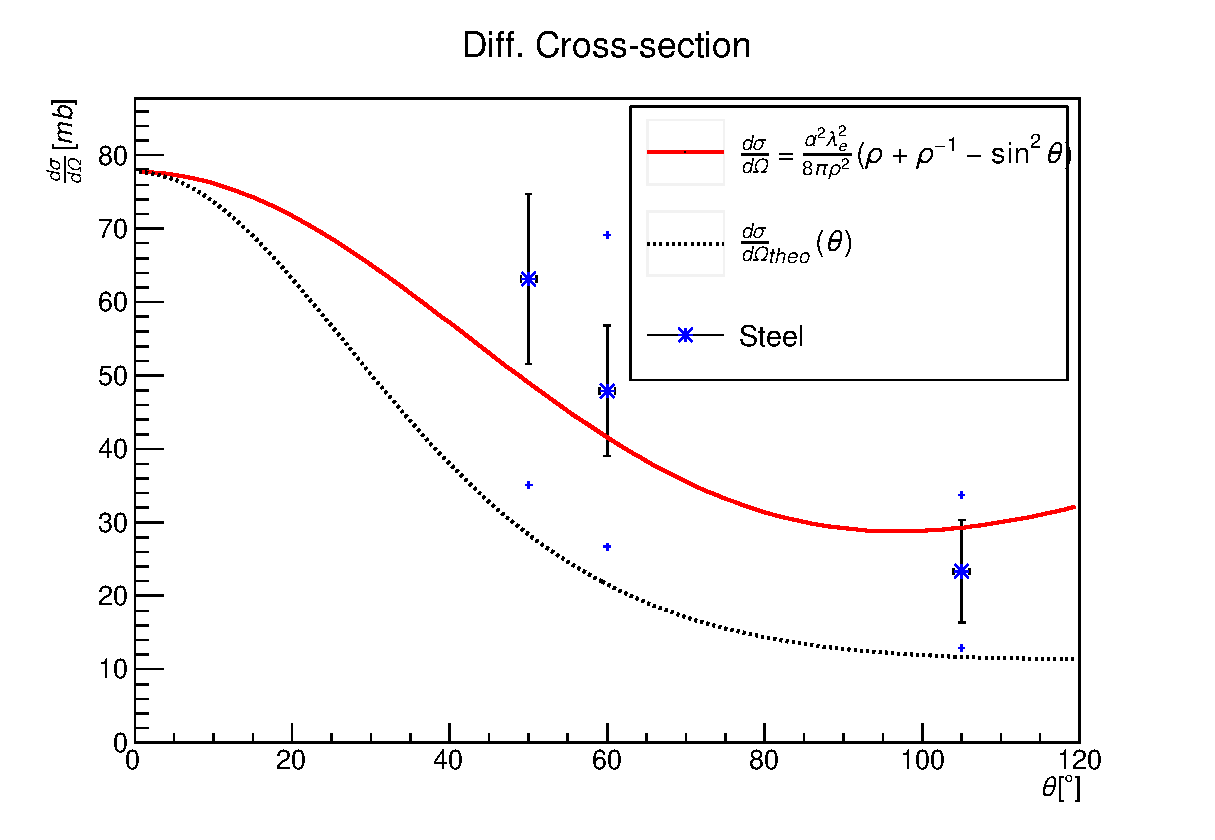
\includegraphics[width=0.9\textwidth]{Graphen/cross-section/diff_cross_Steel_.eps}
    \caption{Differential cross-section of steel and fit to determine the total cross-section again in red. The dotted black curve is again the theoretical differential cross-section. Only the data for 50$^\circ$, 60$^\circ$ and 105$^\circ$ is used, because the others deviate too much.}
    \label{cross_alu}
\end{figure}
\begin{figure}[H]
    \centering
    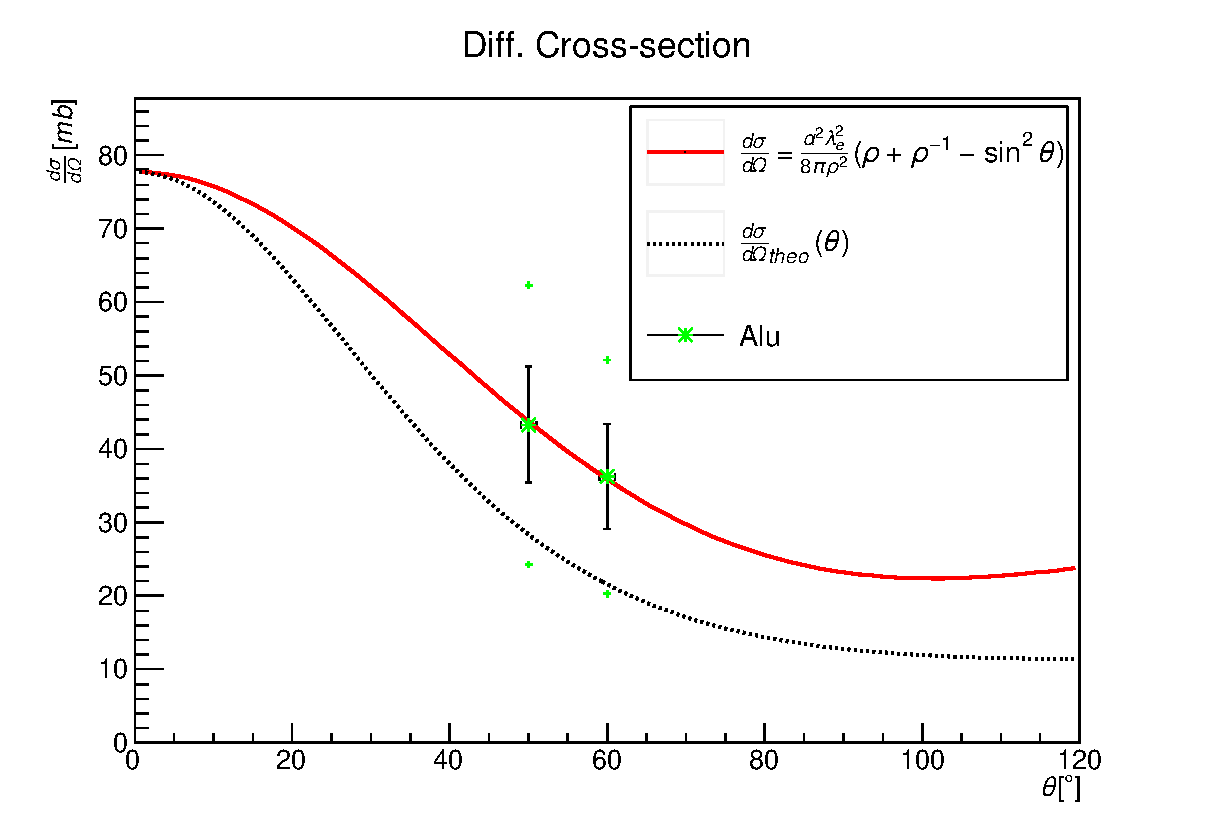
\includegraphics[width=0.9\textwidth]{Graphen/cross-section/diff_cross_Alu_.eps}
    \caption{The same for aluminium. Here only the results for 50$^\circ$ and 60$^\circ$ are used. }
    \label{cross_steel}
\end{figure}
To calculate the total scattering cross-section for conventional geometry, the data of the steel and aluminium scattering body is considered separately. The eq.(\ref{diff_cross}) for the differential cross-section is integrated over all angles to get the total cross-section. The result is
\begin{equation*}
    \sigma_{tot} = \frac{\alpha^2\lambda^2_e}{2\pi}\qty(\frac{2+a(1+a)(8+a)}{(1+2a)^2}+\frac{(a-1)^2-3}{2a}\ln(1+2a))
\end{equation*}
So the values for $a = \frac{E_\gamma}{m_e}$ can be calculated in the fits in fig.(\ref{cross_steel}) and fig.(\ref{cross_alu}), with $\rho = 1+a(1-\cos{\theta})$. The Amplitude dependant on $\alpha$ and $\lambda_e$ is not taken as a parameter, because this value is actually a fundamental constant. The expected values are
\begin{equation*}
    \sigma_{tot, theo} = 251.24\mbox{ mb and } a_{theo} = 1.29
\end{equation*}
The results for aluminium are
\begin{equation*}
    a_{alu} = 0.35 \pm  0.20 \pm  1.31 \mbox{ , } \sigma_{alu} = (411.47 \pm  73.73 \pm 472.22)\mbox{mb}
\end{equation*}
So $a$ deviates $0.71 \sigma$ from the expected value, but only because of the huge systematical error.
This large discrepancy propagates to the total cross-section, deviating $0.33 \sigma$ from the theoretical cross-section.
The quality of the fit is $\chi^2/N_{dF} =1.362$, that seems like a good result, but that is likely due to the large errors of the data points.\\
The results for steel are
\begin{equation*}
    a_{steel} =  0.17 \pm  0.10 \pm  0.94 \mbox{ , } \sigma_{steel} =(499.49 \pm  66.37 \pm 597.53)\mbox{mb}
\end{equation*}
Here the difference between the calculated value of $a$ and $a_{theo}$ is $1.18 \sigma$, but again this is because of the large systematical error, not because the results of the fit are that good.
Another argument for this explanation is the quality $\chi^2/N_{dF} = 0.006$ of the fit. That is way too low, because the fit is performed with only two data points with an immense error.
The values for the total cross-section again differ immense, due to the offset from the theoretical value of the differential cross-section and the calculated one, like mentioned before.\\
That being said the two values for aluminium and steel are actually compatible with respect to the statistical error, indicating they share the same systematic errors.
\subsection{Electron mass}
\begin{figure}[H]
    \centering
    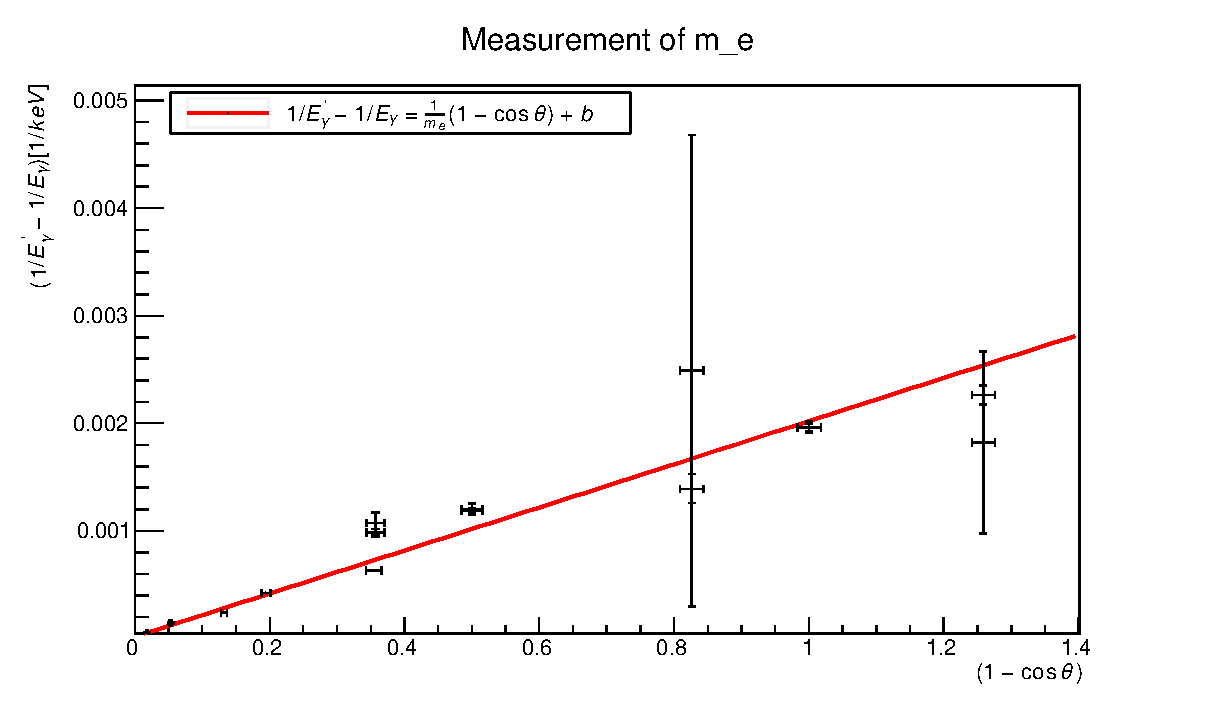
\includegraphics[width=0.9\textwidth]{Graphen/e_mass/e_mass_compton.eps}
    \caption{linear fit to calculate the electron mass. The huge errors in the energy are caused by the difficult peak determining in the data of aluminium.}
    \label{e_mass_compton}
\end{figure}
In this section, again the rest mass energy of the electron is measured by using eq.(\ref{eq_Compton}). If $\frac{1}{E'_\gamma}-\frac{1}{E_\gamma}$ is plotted over $(1-\cos{\theta})$ and a linear function is fitted to the data, the electron mass is the inverse slope. The energy of the Compton scattered photons $E'_\gamma$ is calculated like mentioned before. The fit and data is shown in fig.(\ref{e_mass_compton}). The results are:
\begin{table}[H]
    \centering
    \begin{tabular}{l|l}
        $\frac{1}{m_e}$ & $(2.00404 \pm  0.02592)\cdot 10^{-3}$/keV\\\hline
        $b$ & $(1.65232 \pm  0.37166)\cdot 10^{-5}$/keV \\\hline
        $\chi^2/N_{dF}$ & 10.61
    \end{tabular}
\end{table}
Actually there should not be an offset, because $E_\gamma$ and $E'_\gamma$ should be equal at an angle of 0$^\circ$. But even without scattering, the photon loses energy for example due to absorption, so the offset is allowed. The resulting offset is small anyway, so it is a realistic value not contradicting the presumed theory.\\
The quality of the fit is not the best, which is likely caused by the difficulty of determining the scattered photo peaks in the conventional geometry.\\
The electron mass, calculated by inverting the slope is
\begin{equation*}
    m_e =  (498.99235 \pm  6.45303)\mbox{keV}
\end{equation*}
which deviates about $2 \sigma$ from the theoretical value $m_{e, theo} = 510.99895$keV. So the result is compatible with the expectation, which is a good result, if one think of the difficulties in determining the scattered photo peaks.

\newpage
\section{Conclusion}
Summarising, the measurement of the energy spectra of the different source went quite well, because all photo peaks and even most of the Compton and back-scatter edges where determined and assigned to the different transitions and decays. Also the peaks caused the decay products and the shielding could be matched to theoretical energies, so that in principle those elements could be identified, if they were unknown.\\
The other aspects of the first section, like the calibration, energy resolution and efficiency of the detector are needed to continue with the measurement of the Compton scattering and of the electron mass, to get to know if the setup is suitable for that. With an energy resolution of a magnitude of eV and an efficiency of about 41$\%$, the detector is usable for those purposes.\\
The rest mass energy of the electron is measured in two different ways. At first by measuring the photo peak of the $\beta+$ decay of \ce{^{22}Na} and the second way is by the energy dependency of the photon energy of Compton scattering. The two results are
\begin{equation*}
    m_{e, Na} = (515.92 \pm 17.28)\mbox{ keV and } m_{e,comp} = (498.99235 \pm  6.45303)\mbox{ keV}
\end{equation*}
Both of them are quite near to the theoretical value of $m_{e, theo} = 510.99895$ keV. The one with sodium got a result that is more like the literature value, but its error is about 3$\%$, which is too big for a good experiment.
So actually the calculation of $m_{e,comp}$ went better, because it has an error of 1$\%$ and deviates about 2$\sigma$ from the expectation.\\
The measurement of the photon energy after Compton scattering was difficult for the conventional geometry, because the noise in the measurement was very high even after subtracting the empty measurement. For example the peaks of steel at 80$^\circ$ or for both scattering bodies at 105$^\circ$ were almost not visible. Nevertheless the scattered photon energy has the expected dependency of the scattering angle, because the initial photon energy and electron mass of the fitted function were quite near to the theoretical values.\\
Nevertheless the fit for determining the differential scattering cross-section is not very conclusive.
It seems there is an offset of about 40 mb from the theoretical curve and the statistical uncertainties of the values are significant.
The systematical errors are also huge and since the experiment is not self-performed the uncertainties in the measurement of the experimental setups might be overestimated. It is hard to diagnose these errors for the same reason.
Because of that, the calculation of the total cross-section is of course also not quite successful.

\newpage

\section{Appendix}

\subsection{Sources of literature values}

\begin{enumerate}
    \item Energies and intensities of decays: \url{https://institut2a.physik.rwth-aachen.de/de/teaching/praktikum/Anleitungen/T02_English.pdf}
    \item mass attenuation coefficients: \url{https://www.nist.gov/pml/x-ray-mass-attenuation-coefficients}
    \item data of aluminum: \url{https://en.wikipedia.org/wiki/Aluminium}
    \item data of steel(iron): \url{https://en.wikipedia.org/wiki/Iron}
    \item electron mass: \url{https://en.wikipedia.org/wiki/Electron_rest_mass}
\end{enumerate}


\subsection{Distribution used for edges}
    \begin{align*}
        P(x) &= \int_{a}^{a+d} c\frac{y-a}{d}\cdot\frac{1}{\sqrt{2\pi}\sigma}e^{\frac{(x-y)^2}{2\sigma^2}} dy\\
        &= \frac{c}{2d} \left[ (x-a)\left(erf\left(\frac{x}{\sqrt{2}\sigma}\right) + erf\left(\frac{d-x}{\sqrt{2}\sigma}\right) \right)
        + \sqrt{\frac{2}{\pi}}\sigma \left( e^{-\frac{x^2}{2\sigma^2}} - e^{-\frac{(d-x)^2}{2\sigma^2}} \right) \right]
        % \qyt( ...
    \end{align*}
    
\subsection{Spectra of ring and conventional setup}
\begin{figure}[H]
    \centering
    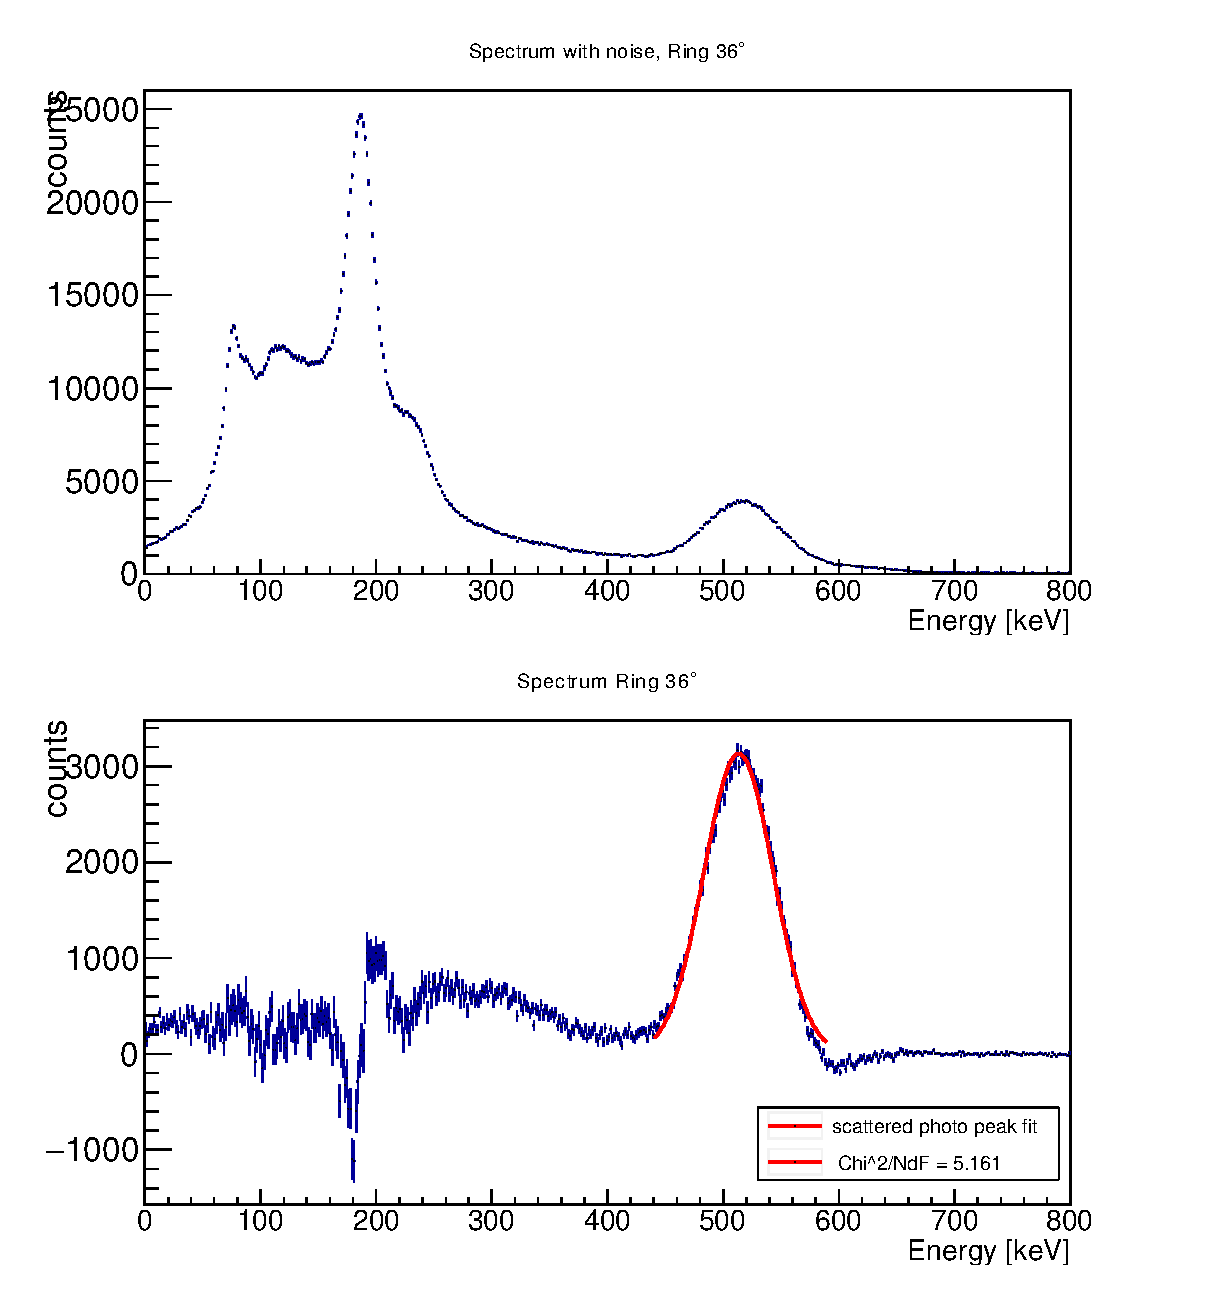
\includegraphics[width=0.9\textwidth]{Graphen/compton_spektren/36grad.eps}
    \caption{}
\end{figure}
\begin{figure}[H]
    \centering
    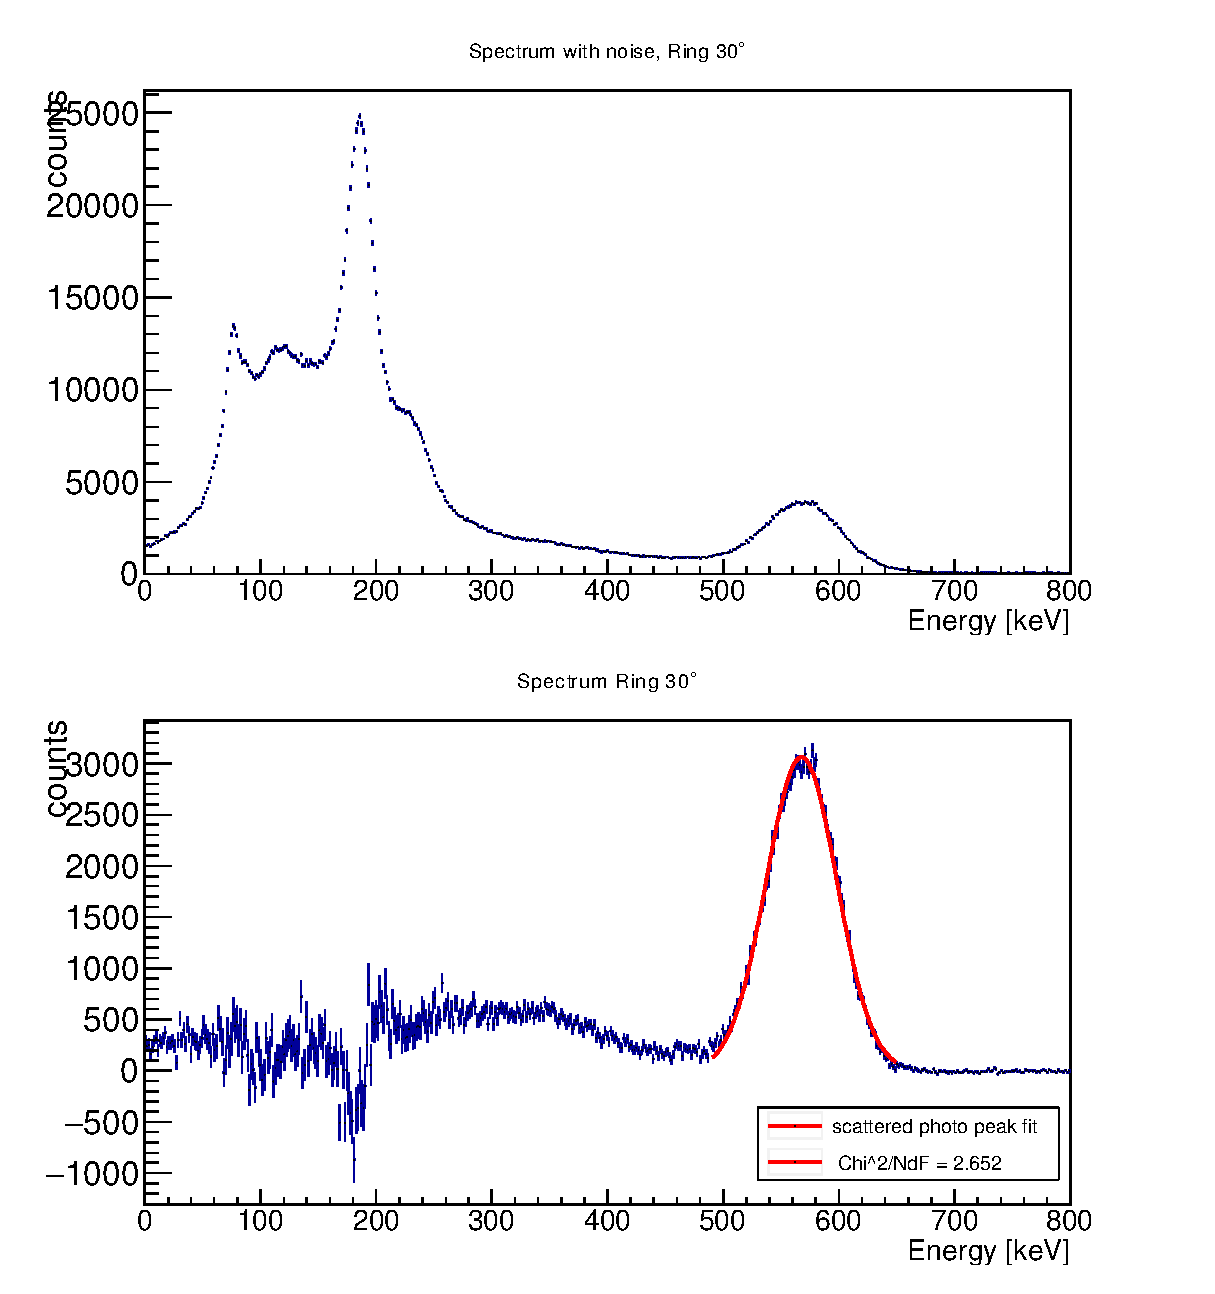
\includegraphics[width=0.9\textwidth]{Graphen/compton_spektren/30grad.eps}
    \caption{}
\end{figure}
\begin{figure}[H]
    \centering
    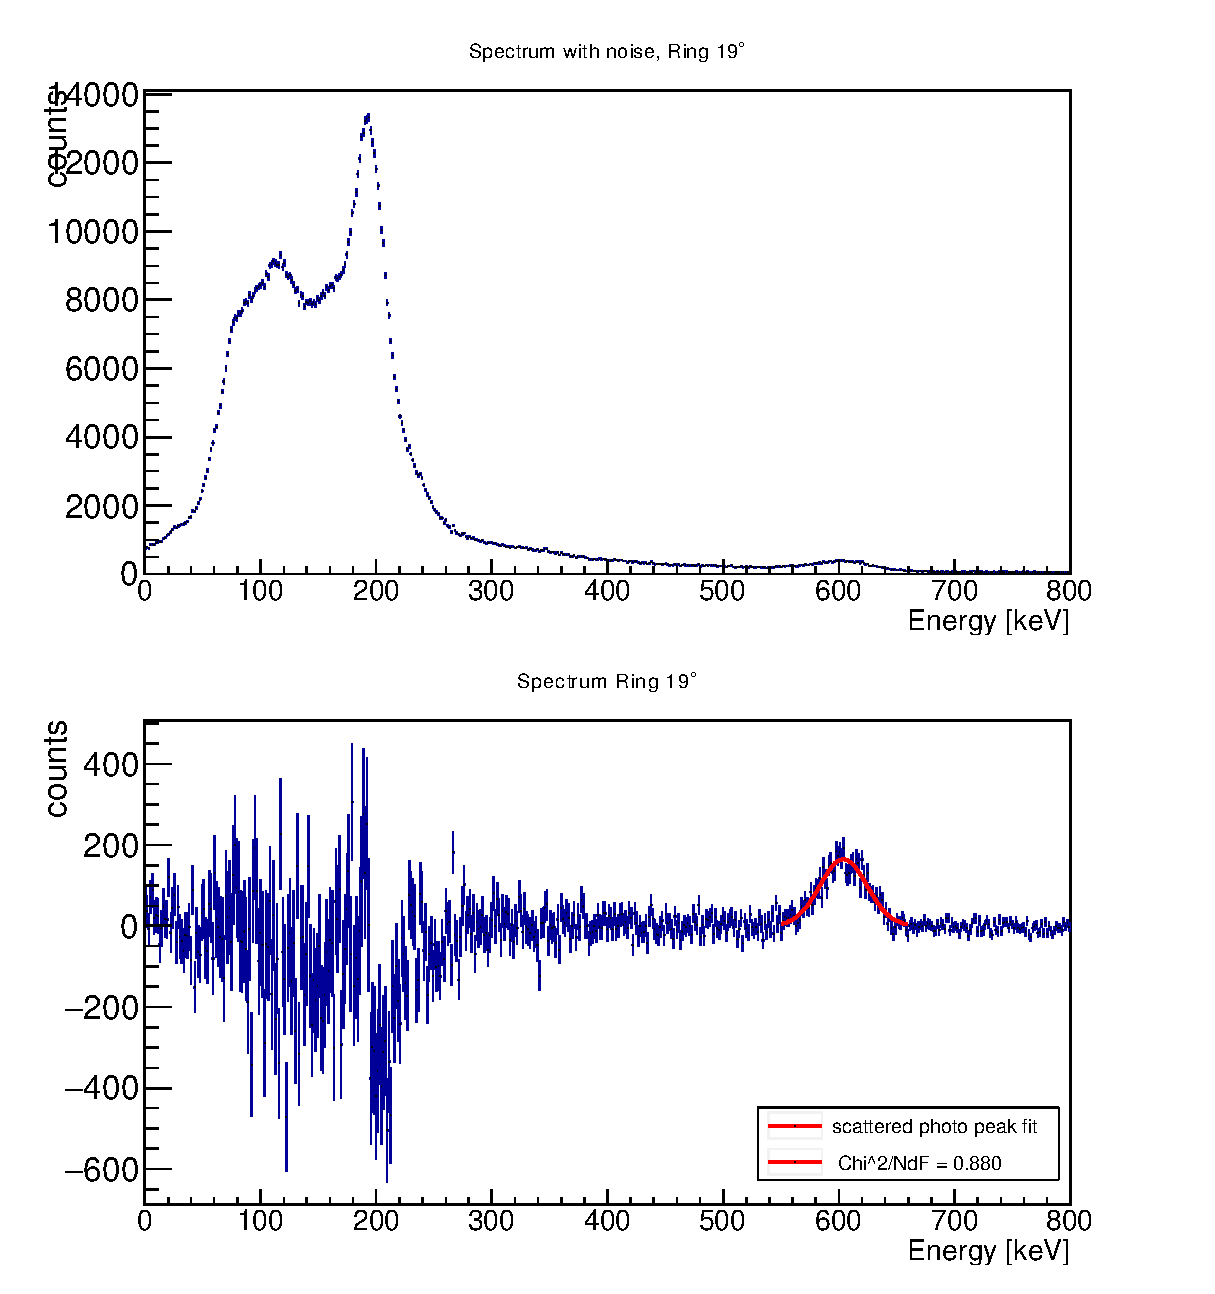
\includegraphics[width=0.9\textwidth]{Graphen/compton_spektren/18,82grad.eps}
    \caption{}
\end{figure}
\begin{figure}[H]
    \centering
    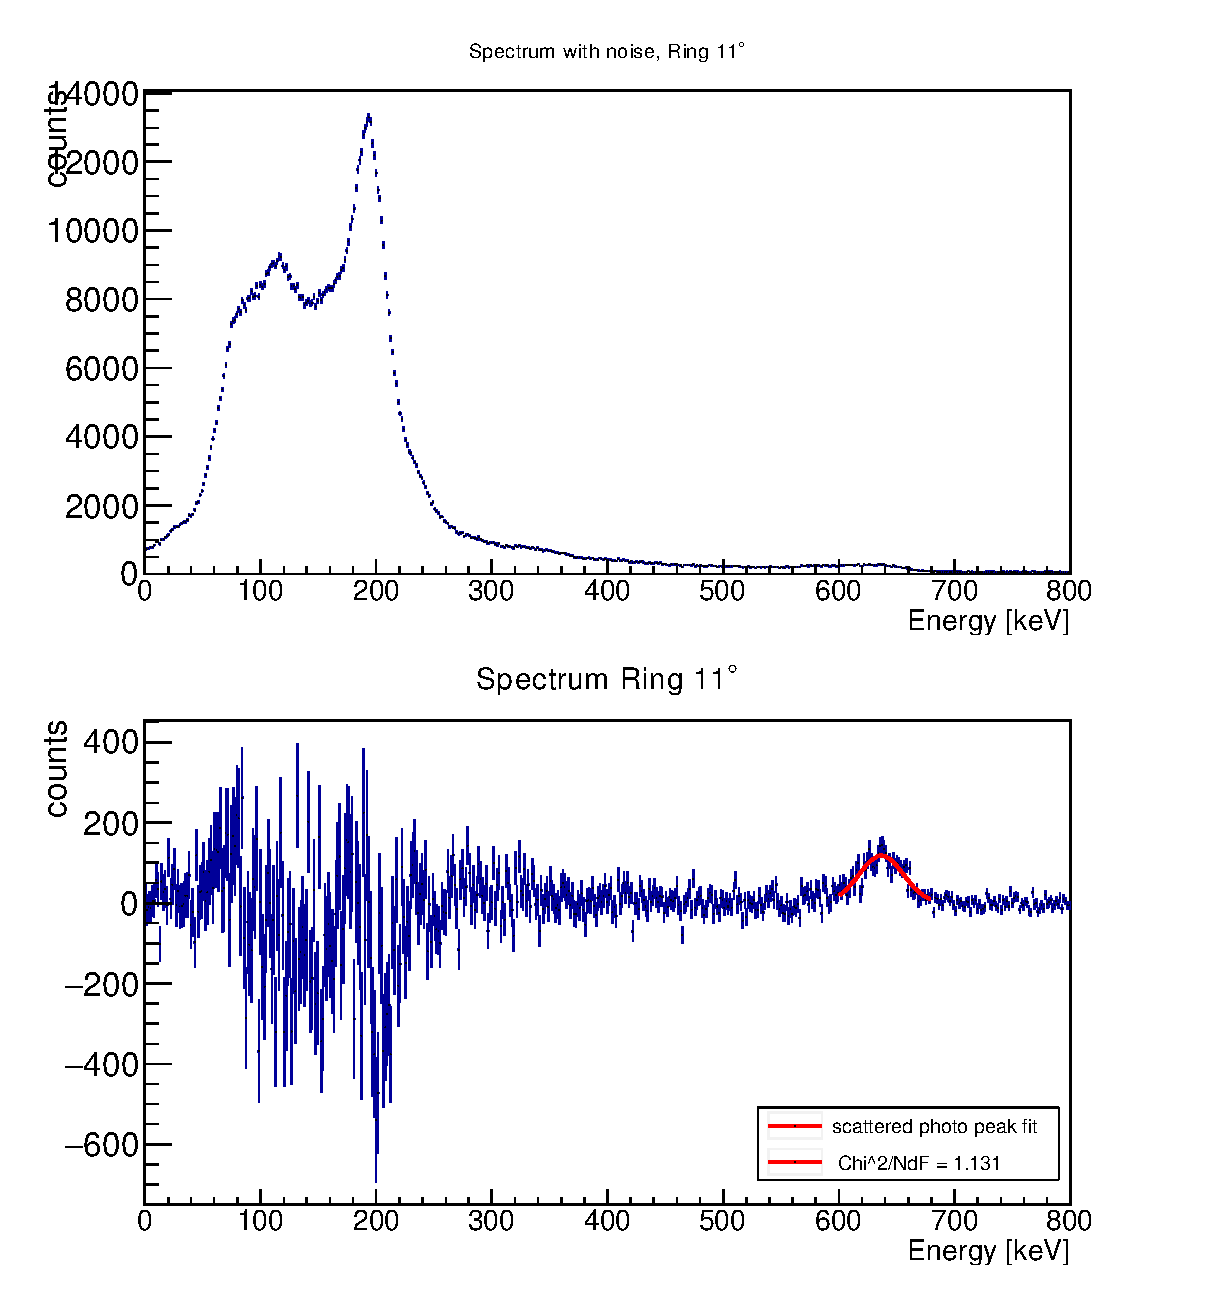
\includegraphics[width=0.9\textwidth]{Graphen/compton_spektren/11grad.eps}
    \caption{}
\end{figure}
\begin{figure}[H]
    \centering
    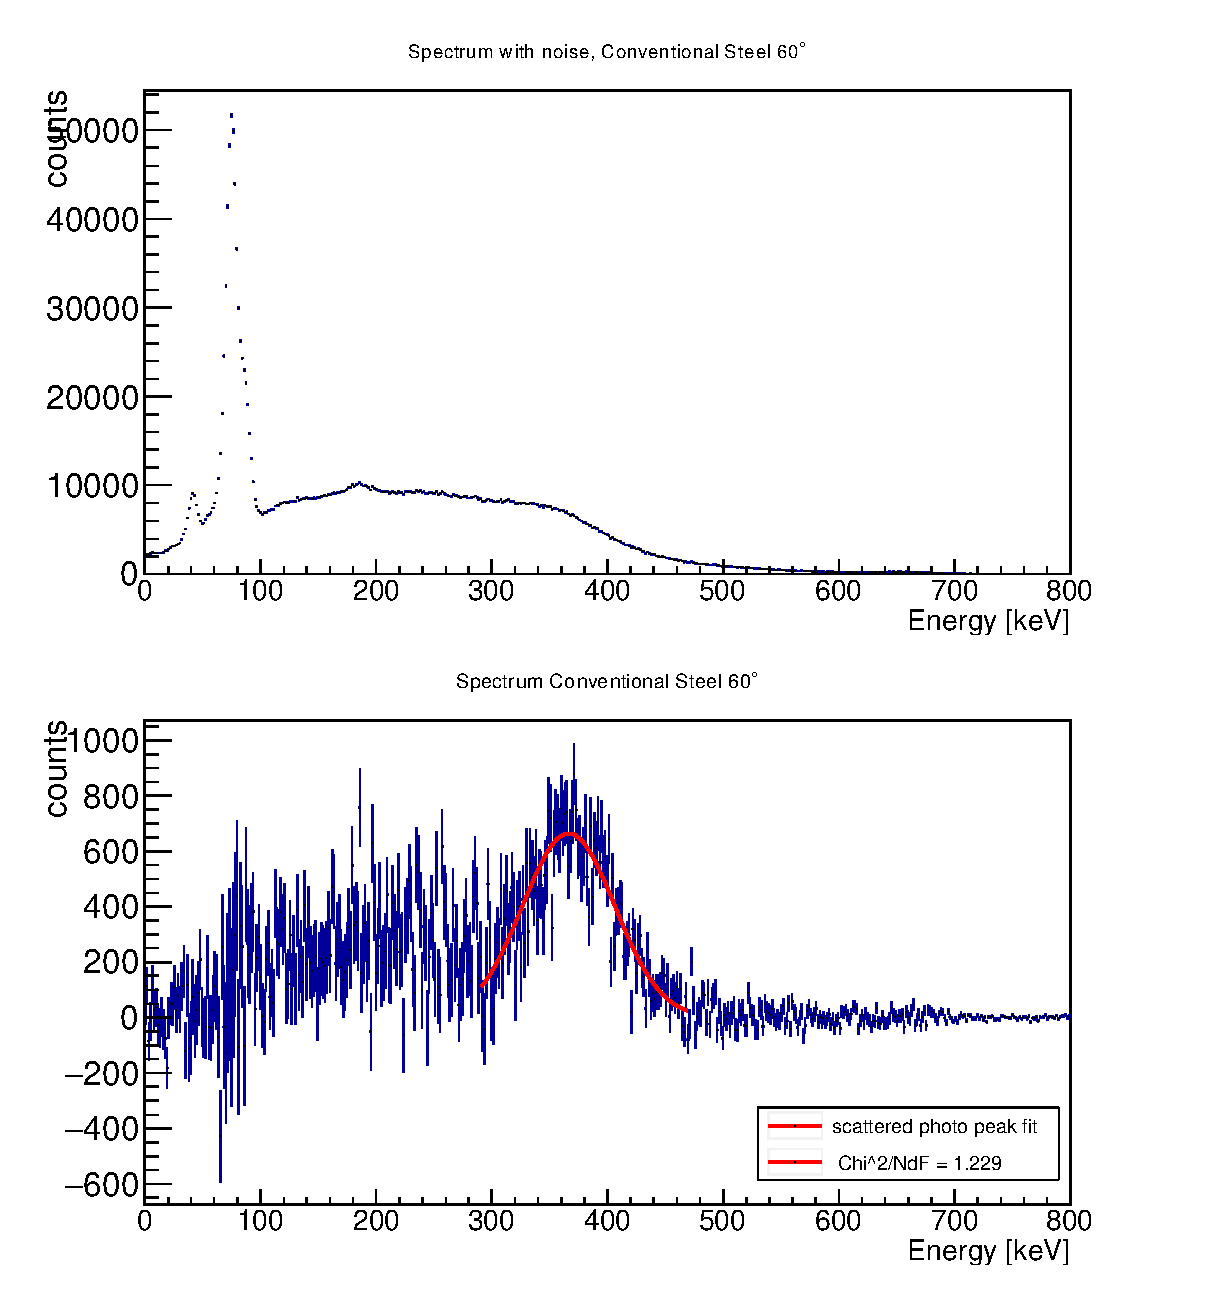
\includegraphics[width=0.9\textwidth]{Graphen/compton_spektren/60Stahl.eps}
    \caption{}
\end{figure}
\begin{figure}[H]
    \centering
    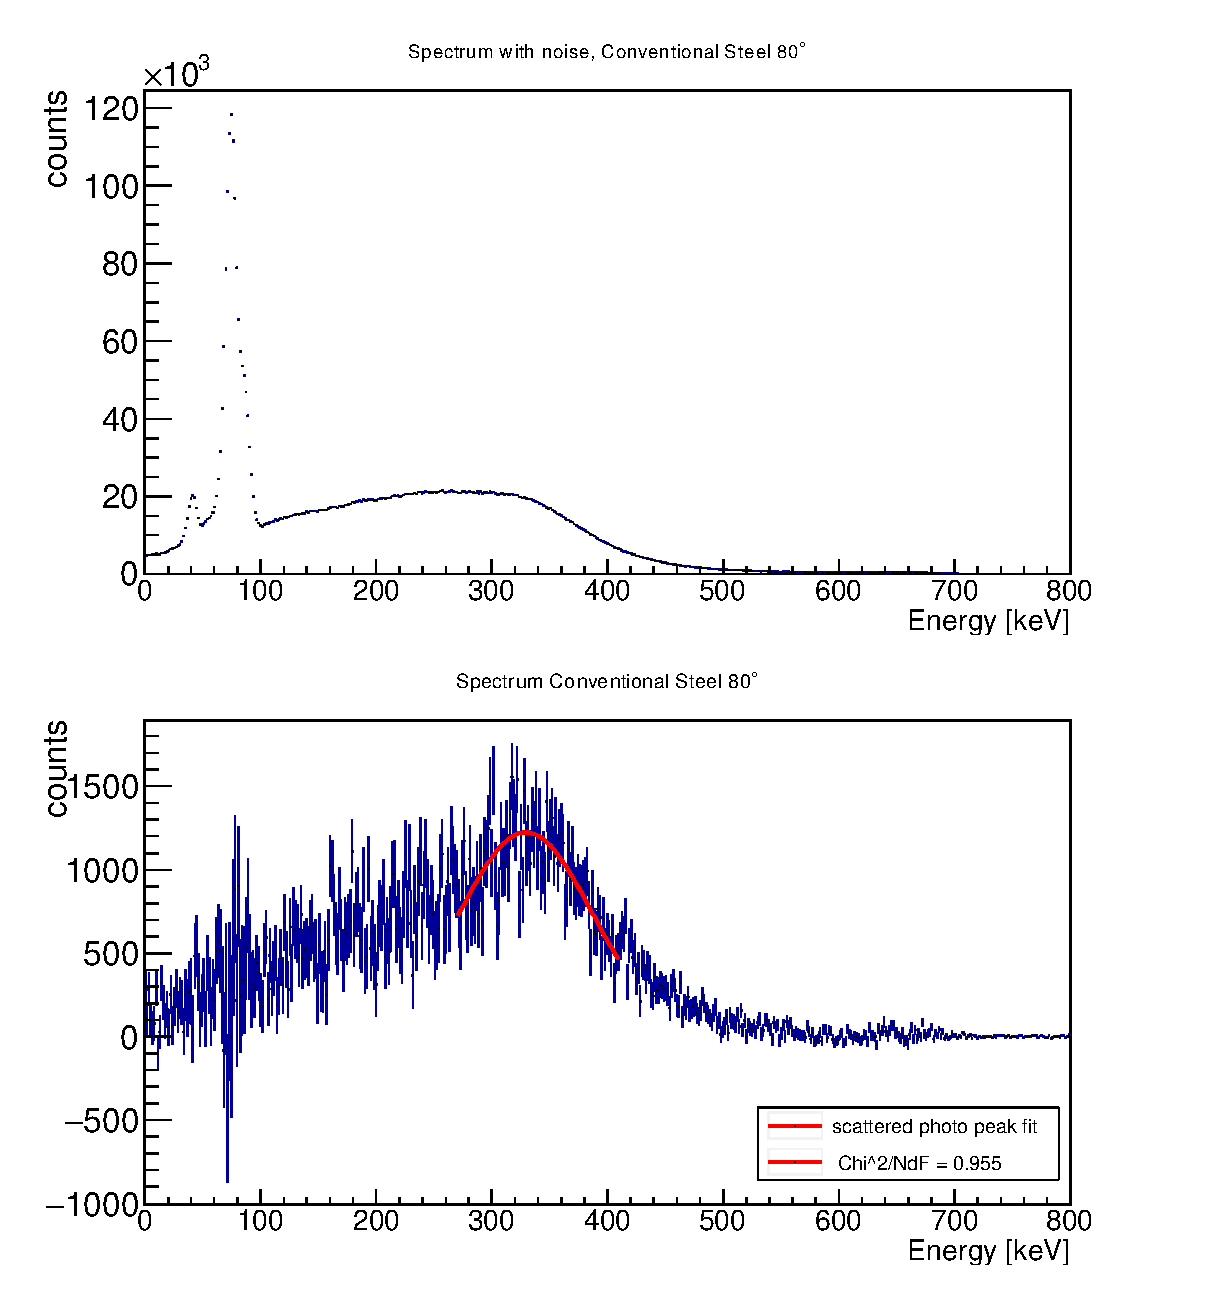
\includegraphics[width=0.9\textwidth]{Graphen/compton_spektren/80Stahl.eps}
    \caption{}
\end{figure}
\begin{figure}[H]
    \centering
    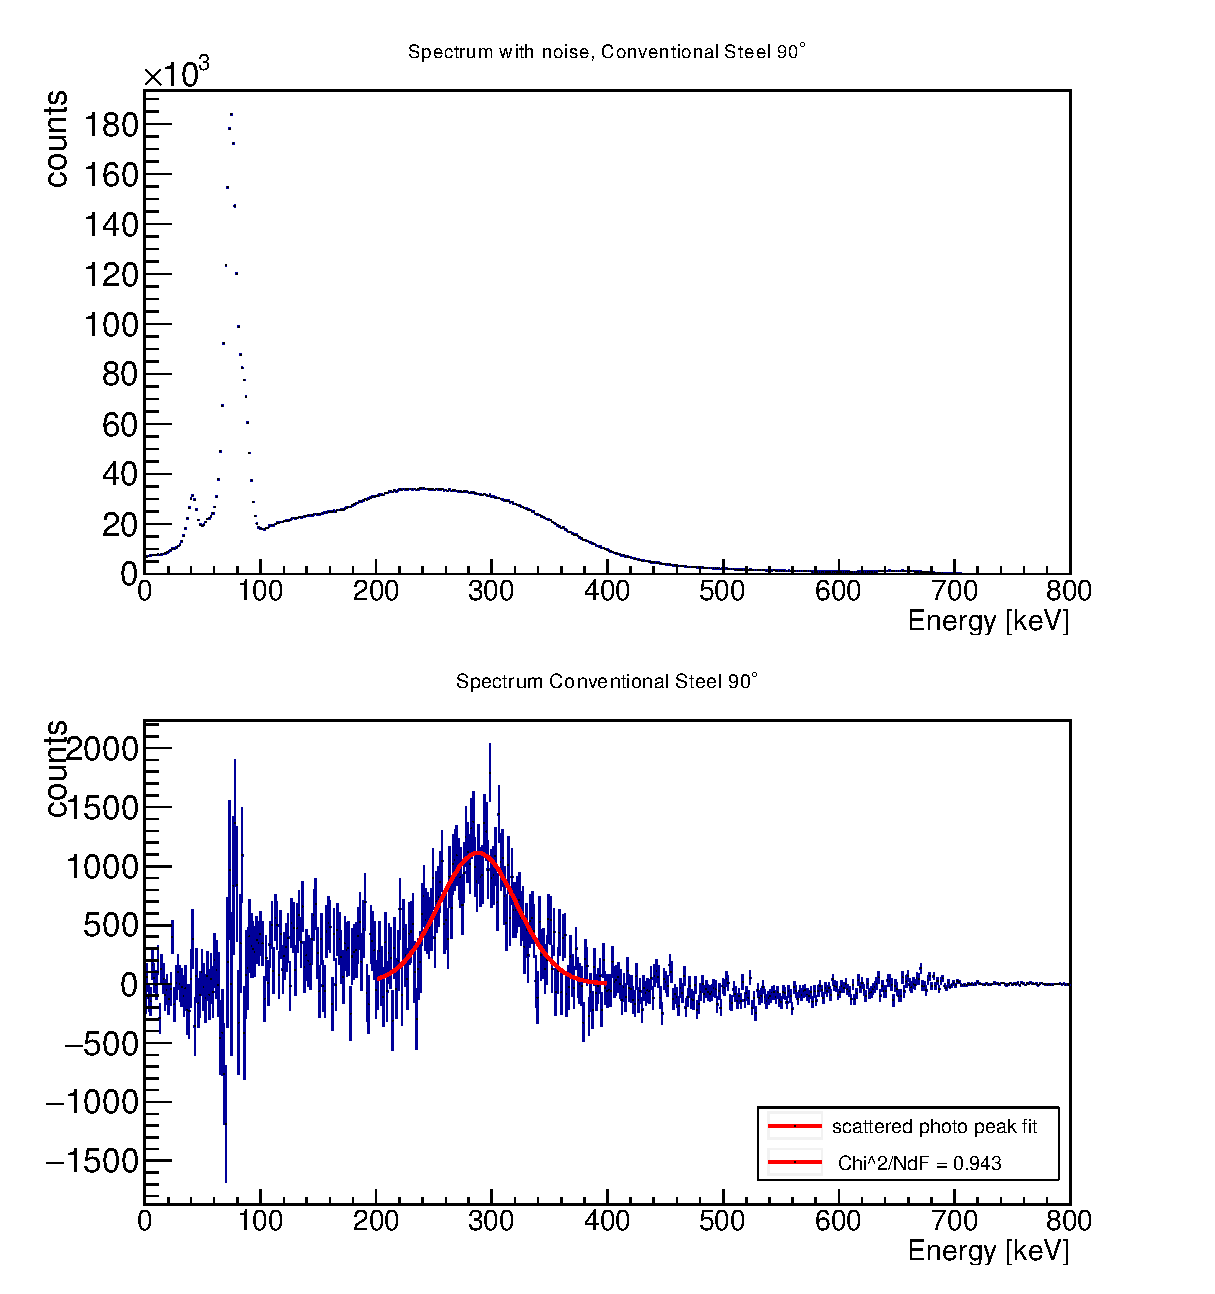
\includegraphics[width=0.9\textwidth]{Graphen/compton_spektren/90Stahl.eps}
    \caption{}
\end{figure}
\begin{figure}[H]
    \centering
    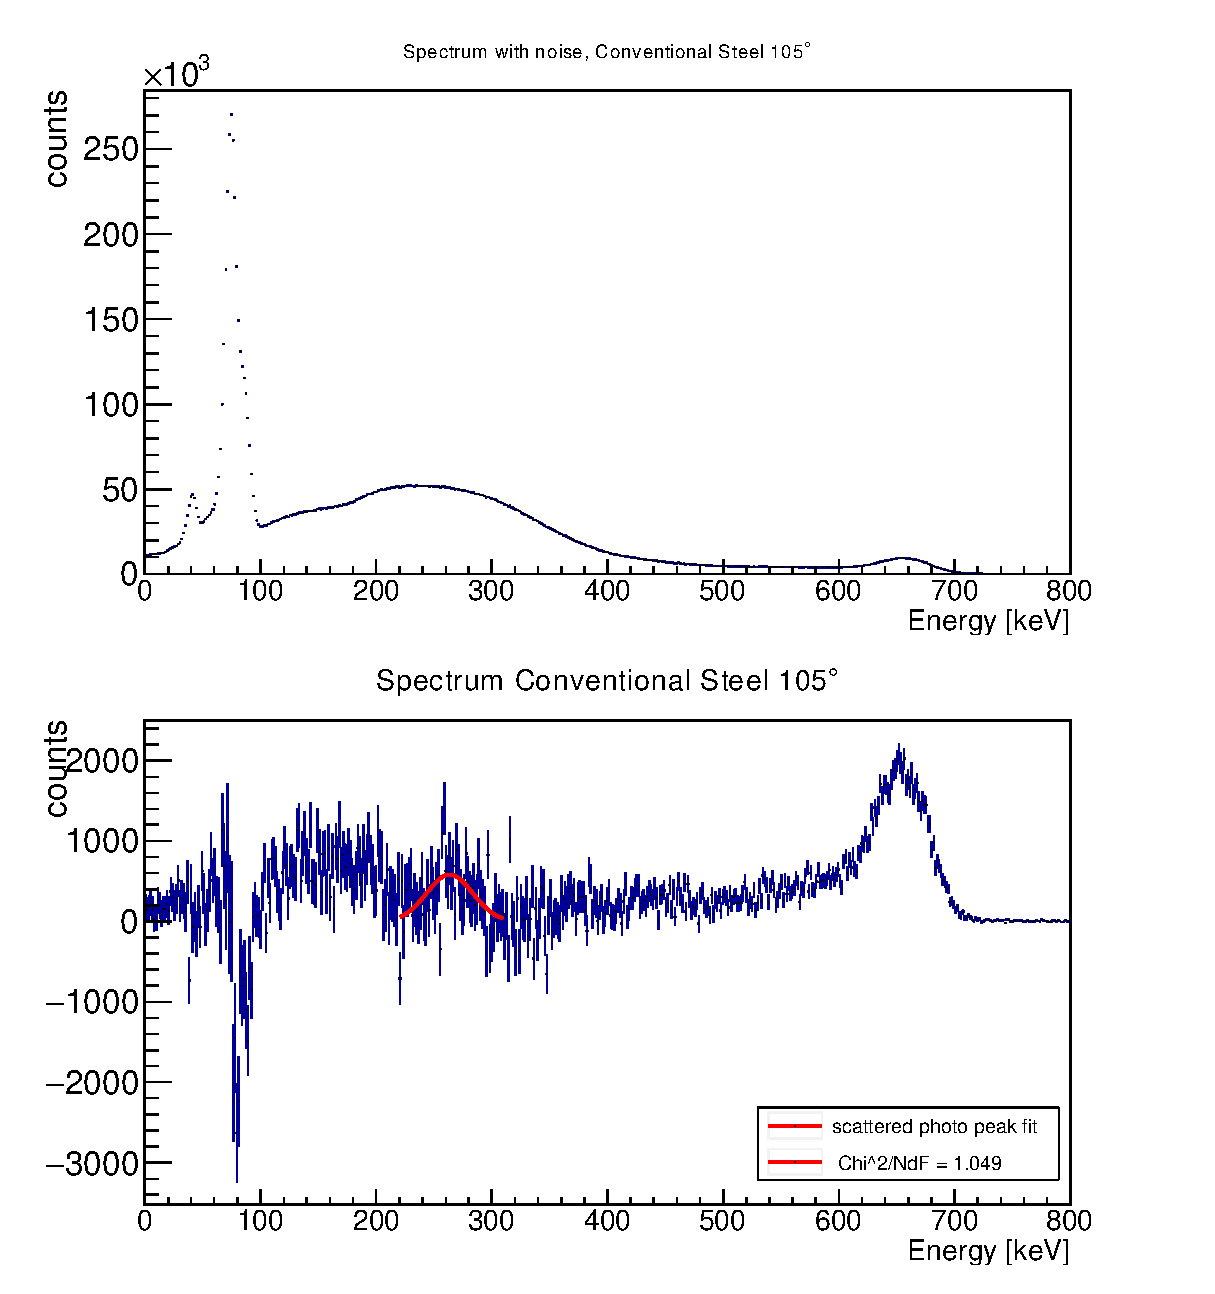
\includegraphics[width=0.9\textwidth]{Graphen/compton_spektren/105Stahl.eps}
    \caption{}
\end{figure}
\begin{figure}[H]
    \centering
    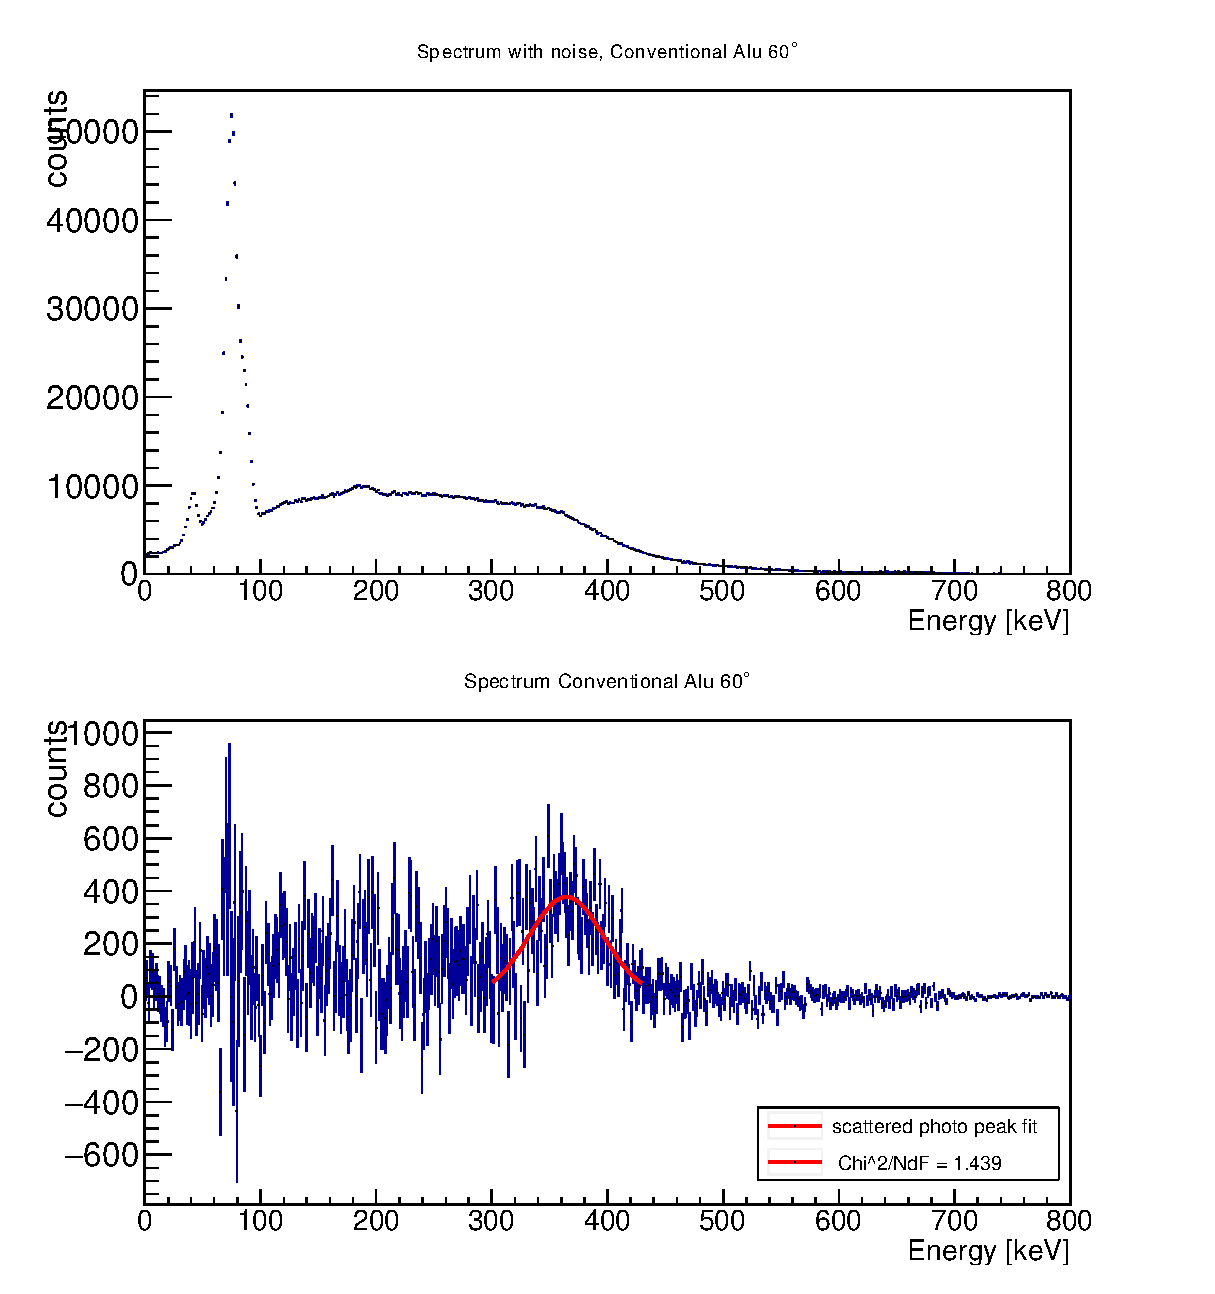
\includegraphics[width=0.9\textwidth]{Graphen/compton_spektren/60Alu.eps}
    \caption{}
\end{figure}
\begin{figure}[H]
    \centering
    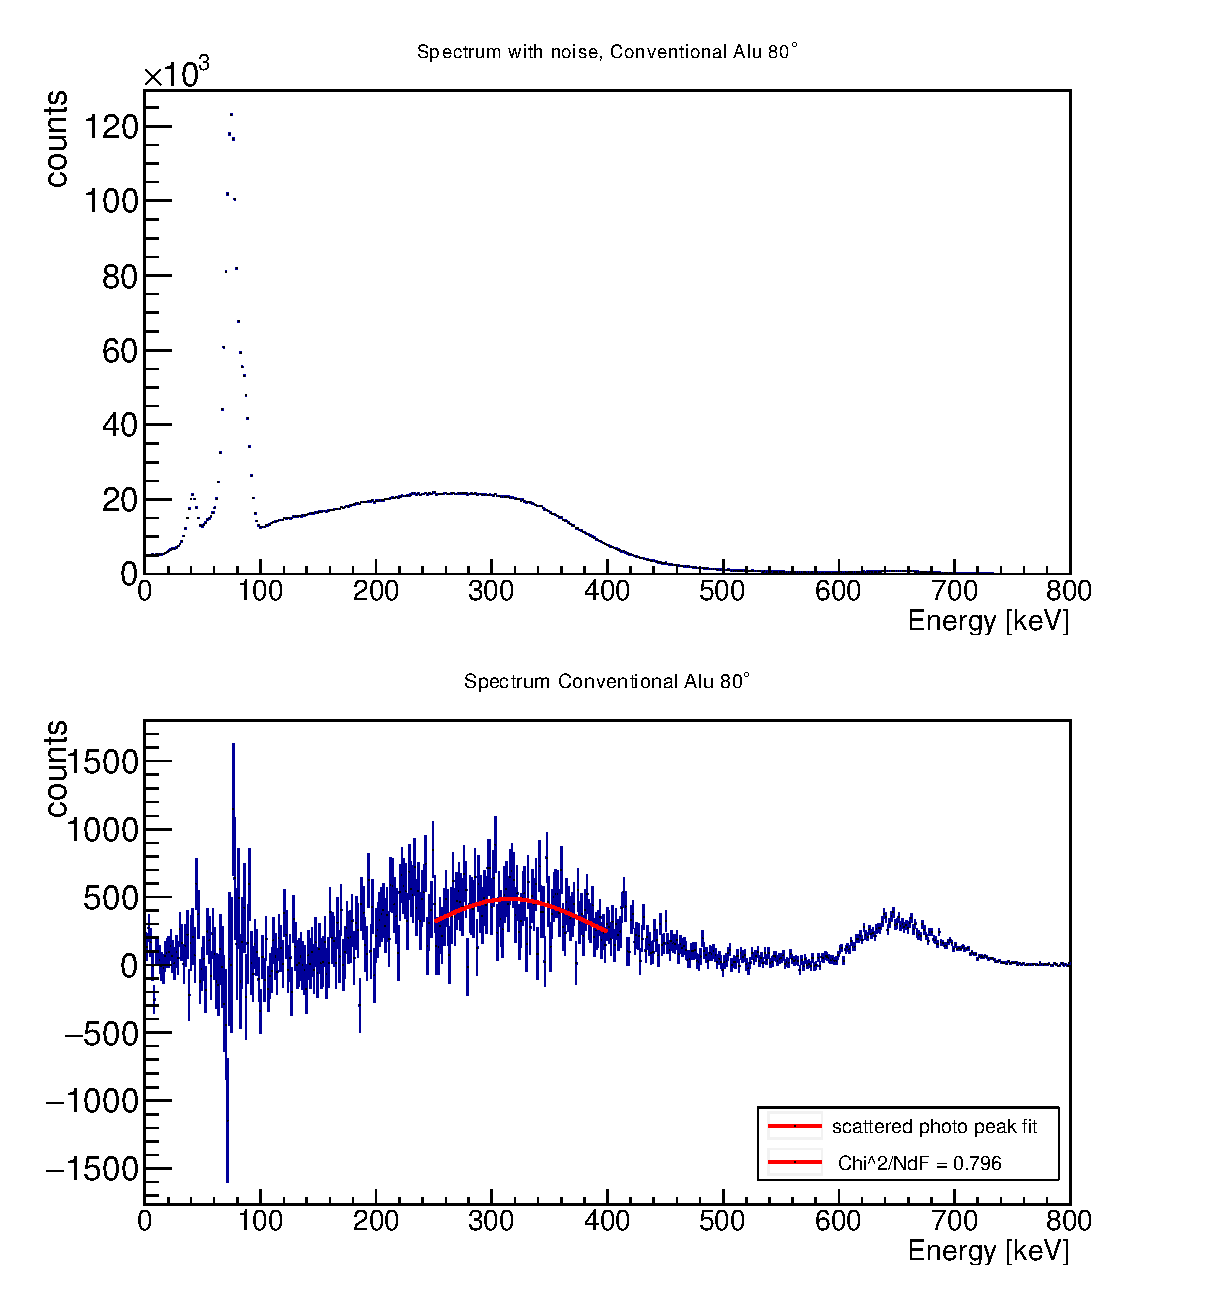
\includegraphics[width=0.9\textwidth]{Graphen/compton_spektren/80Alu.eps}
    \caption{}
    \label{80_alu}
\end{figure}
\begin{figure}[H]
    \centering
    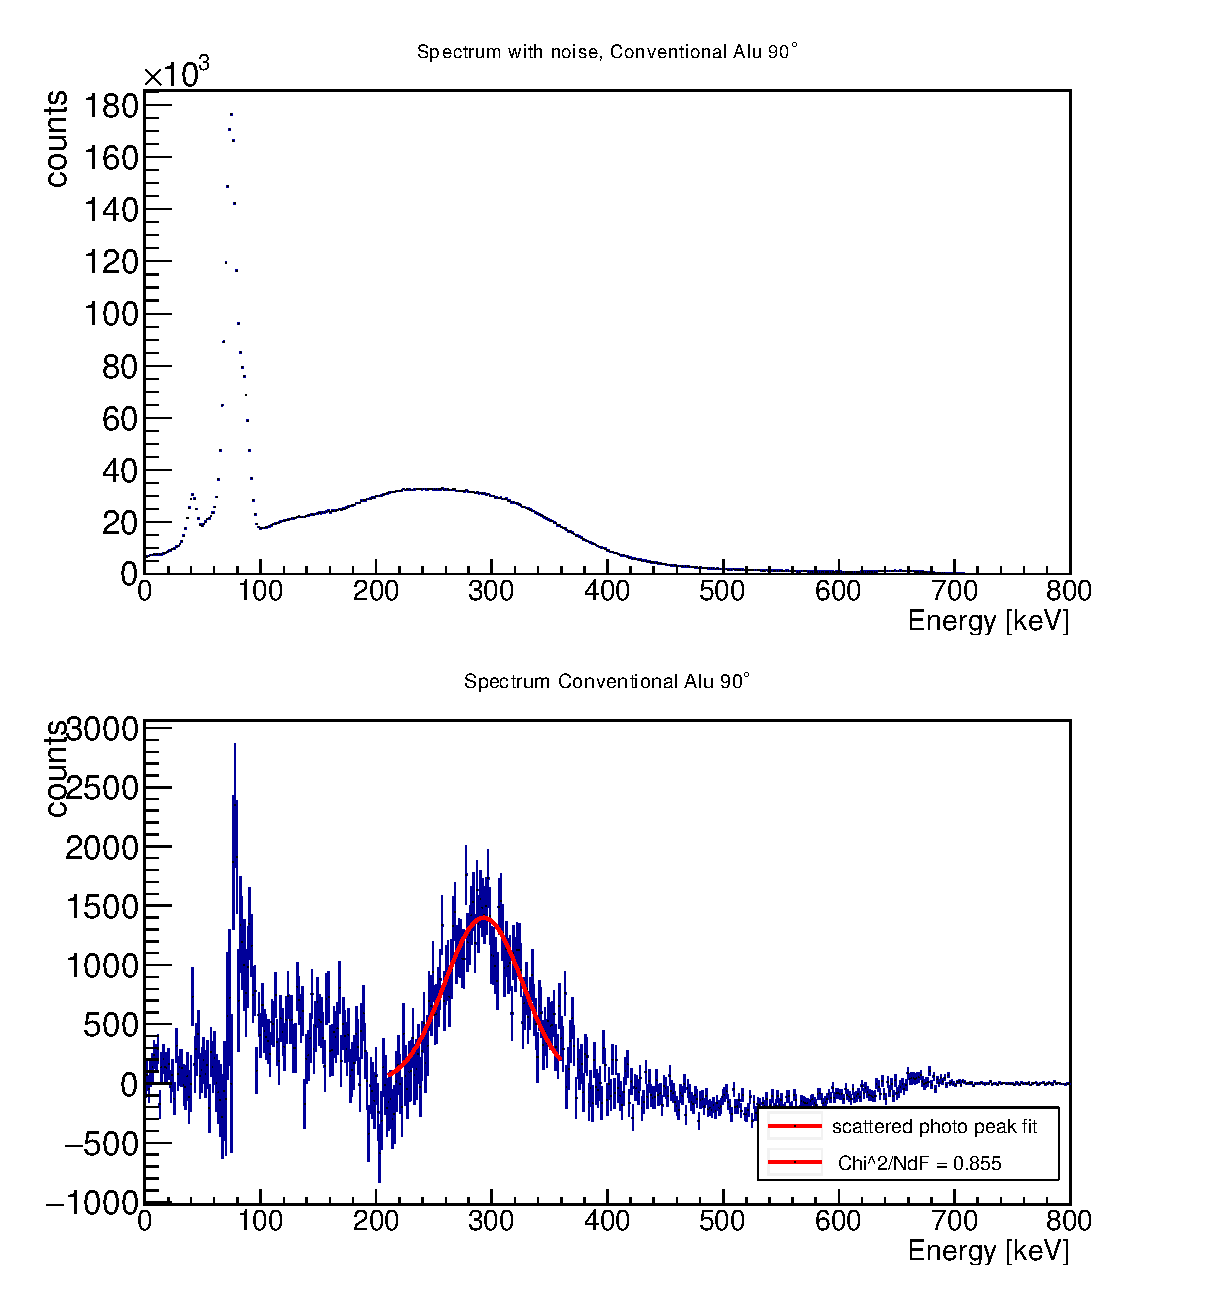
\includegraphics[width=0.9\textwidth]{Graphen/compton_spektren/90Alu.eps}
    \caption{}
\end{figure}
\begin{figure}[H]
    \centering
    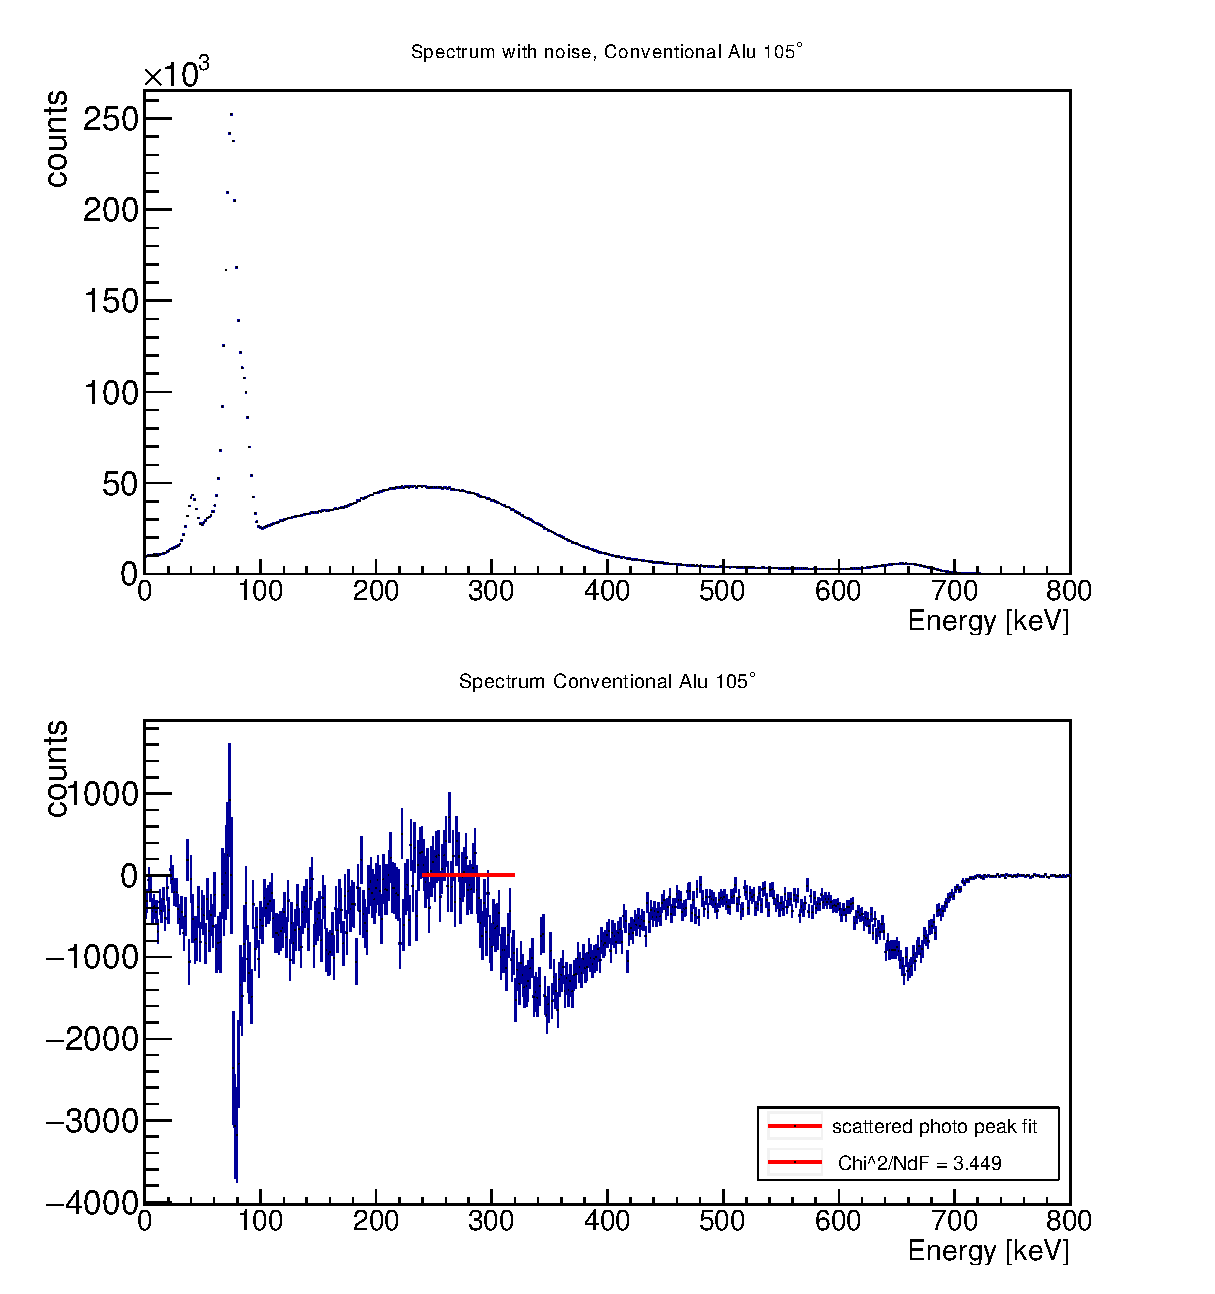
\includegraphics[width=0.9\textwidth]{Graphen/compton_spektren/105Alu.eps}
    \caption{}
\end{figure}


\end{document}

    % \begin{wrapfigure}[13]{l}[0cm]{7cm}
    %    \fbox{\includegraphics[width=7cm]{Bilder/Aufbau1.jpeg}}
    %   \caption{}
    % \end{wrapfigure}

    %\begin{table}[H]
    %\caption{Cassy-Einstellungen Frequenzmessungen}
    %    \begin{tabular}{|l|l|}
    %        \hline
    %        Cassy, Eingang A  & Spannung\\\hline
    %    \end{tabular}
    %\end{table}
    
    %\begin{figure}[H]
    %   \centering
    %    \includegraphics[width=\textwidth]{Graphen/Pendel_B_Roh.eps}
    %    \caption{Rohdaten von Pende} B mit markierten Nulldurchgängen und Auswertungsbereichl
    %    \label{fig:my_label}
    %\end{figure}
    
    %\begin{wraptable}[8]{l}[0.5cm]{5cm}
    %    \caption{Parameter der lin. Reg.}
    %    \begin{tabular}{|l|l|l|}
    %        \hline

    %       \hline
    %    \end{tabular}
    %\end{wraptable}
    

\end{figure}